% $Id: $
\documentclass[a4paper,11pt]{article}
\usepackage{a4wide}
\usepackage{graphicx}
\usepackage{caption}
\usepackage{subcaption}
\usepackage[labelfont=bf]{caption}
\usepackage{enumerate}
\usepackage{amsmath,amsthm,amssymb}
\usepackage{amsfonts}
% The following makes latex use nicer postscript fonts.
\usepackage{times}
\usepackage{subcaption}
\usepackage{datatool}
\usepackage[utf8]{inputenc}
\usepackage{pdflscape}
\usepackage{longtable}
\usepackage{tocloft}
\usepackage{epigraph}

\usepackage[dutch]{babel}
\usepackage{tikz}
\usepackage[toc,page]{appendix}

%\usepackage[colorlinks,urlcolor=blue,linkcolor=blue]{hyperref}
\pagestyle{headings}
\newcommand{\upuparrow}{\mathrel{\reflectbox{\rotatebox[origin=c]{90}{$\twoheadrightarrow$}}}}
\newcommand{\downdownarrow}{\mathrel{\reflectbox{\rotatebox[origin=c]{90}{$\twoheadleftarrow$}}}}
\usepackage{vubtitlepage}
\usepackage{lmodern}
\usepackage{graphicx}

\usepackage[geometry]{ifsym}
%\usepackage[font=small,format=plain,labelfont=bf,up,textfont=it,up]{caption}
\renewcommand{\thefigure}{\thesection.\arabic{figure}}
\author{Filip Moons}
\title{Stagerapport}

\newtheorem{theorem}{Theorem}[section]
\newtheorem{lemma}[theorem]{Lemma}
\newtheorem{proposition}[theorem]{Proposition}
\newtheorem{conjecture}{Conjecture}
\newcommand{\tussen}[1]{\paragraph*{#1}\mbox{}\\}
\newtheorem{property}[theorem]{Property}
\newtheorem{definition}[theorem]{Definition}
\newtheorem{corollary}[theorem]{Corollary}
\newtheorem{remark}[theorem]{Remark}
\newtheorem{remarks}[theorem]{Remarks}
\newtheorem{notation}[theorem]{Notation}
\theoremstyle{definition}
\newtheorem{example}[theorem]{Example}
\newtheorem{examples}[theorem]{Examples}
 \usepackage[table,xcdraw]{xcolor}
\setcounter{tocdepth}{5}
\newcommand{\N}{{\mathbb N}}
\newcommand{\Z}{{\mathbb Z}}
\newcommand{\Q}{{\mathbb Q}}
\newcommand{\R}{{\mathbb R}}
\newcommand{\C}{{\mathbb C}}
\newcommand{\HQ}{{\mathbb H}}
\renewcommand{\P}{{\mathbb P}}
\newcommand{\E}{{\mathbb E}}
\newcommand{\cost}{\text{cost}}
\newcommand{\Nash}{\text{Nash}}
\newcommand{\Tau}{\mathrm{\tau}}
\newcommand{\nash}{\text{nash}}
\newcommand{\opt}{\text{opt}}
\newcommand{\LFP}{\text{LFP}}
\renewcommand{\int}{\text{int}}
\newcommand{\enquote}[1]{`#1'}
%\newenvironment{proof}{\noindent{\bf Bewijs.}}{{\hfill $ \ Box $}\vskip 4mm}

\promotortitle{Titularis}
\promotor{Prof. Dr. L. Van Looy\\}
\advisors{Mevr. Betty Van Bocxlaer (Heemschool)}
\advisortitle{Stagementor:}
\begeleider{Mevr. Evelyne De Smet (VUB)}
\addto\captionsenglish{\renewcommand*\abstractname{Abstract for non-mathematicians}}
\date{MEI 2006}
\faculty{Specifieke Lerarenopleiding}
\advisortitle{}
\department{Wetenschappen \& Ingenieurswetenschappen}
\reason{Verbredende oefenstage - Heemschool}

\date{Februari 2015}


\begin{document}
% Then english TitlePage
\maketitlepage


\tableofcontents
\newpage
\section{Inleiding}
Dit stageverslag bespreekt alle facetten van de Verbredende oefenstage, die ik heb doorlopen op de Heemschool in februari 2015. 
Het stagerapport bevat mijn motivatiebrief, bespreekt de stageschool, de observaties en bevat een zeer grondige toelichting van het uitgevoerde project. 
Daarnaast vindt u ook nog een logboek terug en concluderen we het rapport met enkele kritische beschouwingen. De bibliografie en een afdruk
van de stageovereenkomst sluiten het geheel af. Het verslag 
probeert de lezer een zo goed mogelijk beeld te geven over het doel en de 
werkzaamheden tijdens de stage.
\newpage
\section{Motivatiebrief}
\emph{Deze passage is een letterlijke weergave van de motivatiebrief zoals ingediend op de idlovos.be-website in november 2014.}
\subsection{Wie ben ik?}
Ik ben Filip Moons, 23 jaar en momenteel combineer ik de opleidingen master Wiskunde, master Toegepaste Informatica
en de specifieke lerarenopleiding Wetenschappen \& Ingenieurswetenschappen. Ik heb namelijk een passie voor
Wiskunde, Informatica en het onderwijs. Mijn passie voor het onderwijs ontdekte ik tijdens mijn engagement bij het jeugdwerk waarbij ik zogoed als
elke schoolvakantie mee  kampen begeleid bij Top Vakantie vzw. In juni 2015 studeer ik af in alle opleidingen. De lerarenopleiding is volledig 
afgewerkt, op de verbredende oefenstage en het vak `Pedagogische vraagstukken' 
na. De begeleide en zelfstandige oefenstage deed ik in september, oktober \& 
november van dit jaar op het Koninklijk Atheneum van Etterbeek, in het 5$^\text{de}$ en 6$^\text{de}$ 
jaar ASO.

\subsection{Motivering projectkeuze}
\subsubsection{Persoonlijke meerwaarde}
Voor deze verbredende oefenstage wil ik eens de grenzen van het vertrouwde achter mij laten
en een nieuwe horizon verkennen: alle projecten rond leerlingen met een beperking spreken me aan (zowel het 
project van KI Woluwe, van de Heemschool 1 \& 2 en het project van de Cardijnschool). 
Het lijkt me zeer verrijkend ondergedompeld te worden in de leefwereld van dit type 
leerlingen.\\

\noindent Hoewel de zeer specifieke zorgeisen bij dit type onderwijs niet mogen onderschat worden, denk 
ik dat in dit type onderwijs heelwat kennis te vergaren valt die ook in het reguliere onderwijs zijn nut heeft. Een anekdote om duidelijk te maken wat ik bedoel: ik volgde vijf jaar geleden reeds een cursus bij 
jeugdwerkvereniging `Crefi' over Bijzondere Doelgroepen (Soetewey, 2009).
Deze vorming leerde je als jeugdwerker omgaan met deelnemers uit een bijzondere 
doelgroep met de hoofdfocus op autistische deelnemers of deelnemers 
met ADHD. Het viel me tijdens die vorming op dat heel veel tips die je daar 
meekreeg, ook voor `gewone' deelnemers van pas komen: bied duidelijke structuur aan, 
maak duidelijke afspraken, gebruik geen figuurlijke taal,... allemaal dingen waar 
ook `gewone' deelnemers de vruchten van plukken. Bij een onderdompeling in de 
wereld van het andersvalide onderwijs, lijkt me eenzelfde ervaring mogelijk: 
heelwat dingen die je tijdens zo'n onderdompeling ontdekt zullen waarschijnlijk 
ook nuttig zijn in het reguliere onderwijs. Daarnaast is een bewustwording van 
de specifieke noden in dit type onderwijs bijzonder interessant om je 
onderwijsvisie te verbreden en te verdiepen als toekomstig leraar. Zeker in het licht van de toenemende
drang naar inclusief onderwijs, waarbij andersvalide leerlingen geïntegreerd worden in een reguliere
school, is dit belangrijk (De Witte, 2013).

\subsubsection{Meerwaarde voor de stageschool}
Alle projecten van de stagescholen bevatten ook het ontwikkelen van 
een eigen project. Hoewel de concrete invulling van zo'n project met de 
stageschool moet besproken worden, ben ik van mening dat ik met mijn 
informatica-achtergrond hier echt een waardevolle rol in kan spelen.  Er worden immers heel wat digitale leeromgevingen voor andersvalide leerlingen 
ontwikkeld (Phipps, 2002). Het voordeel van zo'n digitale leeromgeving is dat ze specifiek kan inspelen op 
de noden van de leerling en dat zo'n leeromgeving een gedifferentieerd 
leertraject kan bevatten. \\
\noindent 

Met het ontwikkelen van zo'n digitale leeromgevingen heb ik  
reeds veel ervaring: ik geef er zelfs nascholingen over aan wiskundeleerkrachten. 
Het lijkt me een echte uitdaging om voor een specifiek project zo'n digitale 
leeromgeving te ontwikkelen gericht op leerlingen met bepaalde beperkingen. 

\subsection{Concrete invulling van het project}
\subsubsection{Planning}
Ik was aanwezig op de introductiesessie eind september, deze introductiesessie 
was bedoeld voor studenten die de verbredende oefenstagen afleggen in het 1$^\text{ste}$ 
semester. Vermits ik graag in januari/februari stage zou lopen en ik toch maar 
de lerarenopleiding in juni 2015 finaliseer, heb ik toen in samenspraak met 
mevrouw De Smet afgesproken om me in te schrijven voor de verbredende oefenstage van het 2$^\text{de}$ semester. Dit
geeft de groep studenten van het 1$^\text{ste}$ semester immers meer ademruimte 
om een gepaste examendatum te prikken en laat ook voor mezelf een 
flexibelere stageplanning toe. Concreet zou ik het liefst in de maanden januari \& februari stage lopen.
Hoewel de stage zogoed als aaneensluitend kan verlopen, moet ik wel één examen afleggen in januari. Hiervoor
is een studietijd van maximaal 3 dagen ruimschoots voldoende, dus een grote onderbreking zal dit examen niet veroorzaken. Afspraken rond de data kunnen best met de stageschool zelf gemaakt worden.
\subsubsection{Takenpakket}
Het takenpakket van al deze stageplaatsen omvat participerende observaties en - in 
samenspraak met een leerkracht - het ontwikkelen van een eigen project. Dit moet 
resulteren in een samenhangend dossier met de observatieverslagen, een logboek met de 
planning en tijdsbesteding, een presentatie voor het mondeling examen en 
een verslag met kritische beschouwingen op de opgedane ervaring. In het KI 
Woluwe wordt tevens van de stagiair verwacht dat hij 10 lessen geeft in het 
eigen vakgebied. In elk geval lijken mij de observaties van fundamenteel belang 
om het project te doen slagen en - afhankelijk van de stageschool - 10 
succesvolle en effectieve lessen te kunnen geven. Dit lijkt me ook het ideale 
moment om mezelf bij te scholen door het lezen van boeken rond de thematiek.

\subsection{Verwachting betreffende het verwerven van competenties}
Concreet verwacht ik op deze stageplaats volgende competenties te verwerven:
\begin{itemize}
  \item \textbf{Kerncompetentie 1: Talentontwikkeling}\\
  Als informaticus zal ik allicht in het kader van het project een digitale 
  leeromgeving ontwerpen en realiseren die voor alle leerlingen leerkansen 
  creëert. In de context van het buitengewoon onderwijs verdienen leerlingen met 
  een beperking hierbij een bijzondere aandacht.
 \item \textbf{Kerncompetentie 2: Leerlinggericht}\\
  Het is de bedoeling om met gerichte observaties tijdens het eigen project een 
  positief leefklimaat te stimuleren waarbij de individuele welzijnsnoden van de 
  leerlingen een prioritaire leidraad vormen.
   \item \textbf{Kerncompetentie 3: Reflectief \& onderzoekend}\\
Vanuit een kritisch, reflectieve houding sta ik open voor opmerkingen of commentaar 
van de mentor in deze stageschool. Daarbij krijgt de geschiktheid van 
leermiddelen \& leeromgevingen voor deze doelgroep een bijzondere aandacht.
\item \textbf{Kerncompetentie 4: Participatief \& coöperatief}\\
Ik zal als teamlid \& partner functioneren als stagiair bij het uitvoeren van de 
observaties, het project en de eventueel te geven lessen.
\end{itemize}
\newpage

\section{Stageschool}
\subsection{Adres en algemene info}
\textbf{MPIGO - Heemschool}\\
\noindent 	Koning Albertlaan 181\\
\noindent  1120 Neder-Over-Heembeek\\

\noindent De heemschool is een school voor kleuter-, lager- en secundair buitengewoon 
onderwijs. Aan de school is ook een `heemhotel' gekoppeld dat als internaat en 
tijdelijk opvangcentrum fungeert. 

\subsection{Aangeboden types buitengewoon onderwijs}
\noindent Mijn verbredende oefenstage deed ik in de Heemschool 1, dat is binnen de Heemschool de afdeling
die lager onderwijs aanbiedt. De Heemschool biedt buitengewoon onderwijs van type 2 en type 4. Deze types betekenen 
het volgende:
\begin{itemize}
  \item \textbf{Type 2} Type 2-leerlingen zijn kinderen met een matige tot ernstige 
  mentale handicap. Kinderen met een type 2-attest hebben een matige tot 
  ernstige mentale retardatie met een IQ lager dan 50 (het algemene bevolkingsgemiddelde is een IQ van 
  100). Het merendeel van de leerlingen op de Heemschool zijn type 2-leerlingen.
  \item \textbf{Type 4} Type 4-leerlingen zijn kinderen met een fysieke of een motorische 
  beperking.
\end{itemize}
\subsection{Onderwijsproject}
\noindent De lagere school tracht voornamelijk de zelfredzaamheid en zelfstandigheid van 
de leerlingen in de mate van het mogelijke te verhogen. De klasgroepen zijn dan 
ook erg klein (gemiddeld 8 leerlingen per klas, t.o.v. 22 per klas in een reguliere lagere 
school) en de leerkrachten worden bijgestaan in hun opdracht door een
gespecialiseerd zorgteam met logopedisten, kinesitherapeuten, ergotherapeuten en
verpleegkundigen.\\
\subsection{Verdeling in klasgroepen}\label{klasgroepen}
\noindent Er zijn verschillende soorten klasjes: je hebt stimuliklasjes, de 
HOE-groep en een autiwerking. Dit betekent het volgende:
\begin{itemize}
  \item \textbf{Stimuliklas} Stimuliklassen zijn klassen met leerlingen met een erg 
  zware mentale beperking, soms gecombineerd met een fysieke of motorische beperking. De naam `stimuli' duidt dan ook op het zoveel mogelijk prikkelen van de leerlingen
  door contact via de zintuigen (visuele prikkels, geluidsprikkels,...). Deze leerlingen komen meestal nooit tot spreken 
  en komen qua cognitief ontwikkelingsniveau overeen met baby's in hun eerste 
  levensmaanden. In de klas doet men aan snoezelen, geluidsspelen, 
  gevoelsoefeningen,...
  \item \textbf{HOE-groep}
  De HOE-groep is een combinatie van klassen met leerlingen met een gematigde 
  mentale beperking en/of fysieke handicap. De HOE staat voor:
  \begin{itemize}
        \item \textbf{Heemklas} De heemklas zijn klasjes waarin eenvoudige leeractiviteiten 
    plaatsvinden. Denk aan activiteiten rond leren naar de winkel gaan (als ze kassierster 2,5 euro vraagt, leren zij dat
    ze 3 euro moeten geven), kloklezen, eenvoudig leren schrijven (dit is niet dezelfde schrijfmethode als in het reguliere lager onderwijs) 
    en lezen op herkenning (zij leren geen letters individueel lezen, maar proberen woorden als een geheel te 
    herkennen). Leerlingen zitten vaak, afhankelijk van hun leeftijd en ontwikkeling, een 2 à 3-tal 
    jaar in de heemklasjes en monden dan meestal uit in de `sterke' eindklas. 
 


   \item  \textbf{Observatieklas}  De observatieklas is een startklasje voor de jongste 
   leerlingen waarin eenvoudige leeractiviteiten plaatsvinden (gezelschapspelletjes spelen, leren zelfstandig aankleden, de dagen/maanden 
   leren,...). De observatieklasjes zijn een opstap naar de heemklassen.
       \item \textbf{Eindklas} De eindklasjes zijn de klasgroepen waarin leerlingen 
    voorbereid worden op de overgang naar het buitengewoon secundair onderwijs (vaak is dat gewoon terug in de Heemschool, die ook een middelbare
    afdeling heeft). Er zijn op dit moment twee eindklasjes: een `zwakke' en 
    `sterke' klas. In de sterke klas komt men min of meer tot een eindniveau dat 
    vergelijkbaar is met dat van een eerste leerjaar in het reguliere lager 
    onderwijs. In de zwakkere klas is dat eindniveau niet echt bepaald en 
    afhankelijk van het kind zelf. In de zwakkere klas kan men activiteiten 
    verwachten zoals werken rond verhalen (luisteren, een scène tekenen,...), 
    knutselen, samen spelen. De zwakkere klas heeft voornamelijk type2-leerlingen die maar heel 
    beperkt zullen socialiseren in de maatschappij en altijd sterk hulpbehoevend 
    zullen blijven. 
   \end{itemize}
  
  \item \textbf{Autiwerking} De autiwerking is in de Heemschool een aparte gang met 
  enkele klassen met uitsluitend autistische leerlingen met een mentale beperking. De 
  niveau's zijn enorm verschillend (sommige komen tot schrijven, lezen en rekenen op een vrij hoog niveau, anderen komen zelfs niet tot 
  spreken) waardoor de begeleiding hier bijna individueel per leerling gebeurt. 
 
\end{itemize}
\subsection{Schoolloopbaan \& toekomst van leerlingen}
Belangrijk op te merken is dat de indeling van leerlingen in een klasgroep jaar 
naar jaar beslist wordt op basis van leeftijd en cognitief ontwikkelingsniveau. 
Het kan gerust zijn dat een leerling meer dan 1 jaar in dezelfde klas blijft. Ook 
de overgang naar het buitengewoon secundair onderwijs is niet louter leeftijdgebonden 
maar wordt voor elke leerling in de eindklas individueel beslist. Zo zat er nog een 
15-jarig meisje in de sterkere eindklas toen ik ging observeren. \\

\noindent De finaliteit van deze leerlingen in het leven als volwassene (dus na het buitengewoon secundair onderwijs) 
valt grofweg uiteen in twee groepen: de meeste leerlingen met een matige mentale 
beperking worden opgeleid om later in een beschutte werkplaats te kunnen werken 
en beschermd of begeleid te wonen. De andere leerlingen met een zware fysieke 
en/of mentale beperking zullen allicht terechtkomen in een tehuis of een sterk beschermde woonplaats. 

\newpage
\section{Observaties}\label{observaties}
Tijdens de observatieweekjes ben ik in totaal een kleine schoolweek gaan 
observeren in de verschillende klasgroepen die beschreven zijn in paragraaf \ref{klasgroepen}. Om de exacte tijdstippen en tijdspanne te weten, verwijs ik door 
naar het logboek in sectie \ref{logboek}. De enige klasgroep die ik niet bezocht 
heb, zijn de stimuliklassen (zeer zwakbegaafde leerlingen met een cognitief ontwikkelingsniveau van een baby in zijn eerste levensmaanden), omdat mijn project rond informatica voor hen sowieso 
te hoog gegrepen zou zijn. Ik beschrijf hier mijn ervaringen tijdens het 
observeren per klasgroep en formuleer nadien een algemene conclusie.

\subsection{Klasgroepen}
\subsubsection{Eindklas 1 - Wendy}
De eindklas 1 van Wendy heb ik enkele keren gaan observeren. Dit is de zwakkere 
eindklas met leerlingen die wel kunnen spreken en goed communiceren, maar voor de rest niet zoveel 
zelfredzaamheid kennen. Ik heb bij Wendy een les gevolgd dat startte met een 
verhaal over Tito De Clown (het was de week rond carnaval), waarna vervolgens de 
leerlingen een kleurplaat moesten inkleuren. Het viel op dat de meeste leerlingen, ondanks hun leeftijd van gemiddeld
11 à 12 jaar, amper binnen de lijnen konden kleuren. Ik heb bij hen ook een 
lesje gevolgd op de computer waarbij de leerlingen hun naam moesten typen. Eén 
leerling was hier erg goed mee weg, maar de overigen konden nauwelijks een 
juiste letter typen. Ik heb zelfstandig samen met een leerling gewerkt, maar hij 
vergat telkens opnieuw waar de toetsen zich ongeveer situeerden. De leerlingen 
waren wel erg aanhankelijk en altijd super enthousiast om mij te zien.

\subsubsection{Eindklas 2 - Kathleen}
De eindklas 2 ben ik een voormiddag gaan observeren op het einde van mijn observatieweekjes. 
Hier viel het meteen op hoe hoog het niveau lag: de leerlingen leerden technisch 
rekenen tot 100 (dus rekenen zonder contexten - bijvoorbeeld naar de winkel gaan - maar echt puur cijfers) 
en konden dat vrij behoorlijk. Heel opvallend was wel dat de meesten stiekem op 
hun handen bleven tellen van zodra dat kon. Toch kwam het niveau ongeveer overeen met een eerste leerjaar van het reguliere basisonderwijs. 
Er was wel één leerling met een fysieke beperking die dit niveau duidelijk niet 
haalde, maar de leerkracht heeft nadien uitgelegd dat hij vooral vanwege zijn 
leeftijd (14 jaar) bij deze groep mocht aansluiten omdat het leeftijdsverschil 
in andere klasgroepen echt te groot zou zijn.
Dit waren ook de oudste leerlingen in de lagere school, met als uitschieters
leerlingen van 14 en 15 jaar. Zij waren ook het minst aanhankelijk van alle klasjes.\\

\noindent Na de geobserveerde les heeft de leerkracht mij allerlei dingen over de klas 
verteld, maar het meest opmerkelijke verhaal was ongetwijfeld dat van een 
leerling met het syndroom van Pradar-Willi. Dat is een genetische afwijking 
dat een constant gevoel van honger veroorzaakt (het syndroom veroorzaakt daarnaast nog tal van andere mentale en fysieke 
problemen). Door dat gevoel van honger, gaan Pradar-Willi's constant op zoek 
naar eten en stelen ze meestal al het eten wat ze tegenkomen. In erg laagbegaafde gevallen (mentale retardatie komt bijna bij alle Pradar-Willi's voor) gaan ze zelf
zo ver dat ze giftige stoffen opeten (papier, karton, krijt, zware metalen,...) waardoor veel Pradar-Willi's op jonge leeftijd sterven. De leerling in 
deze klas zat ook op internaat in het Heemhotel en stond hier op een zeer sterk gecontroleerd eetregime. Ze werd ook elke dag gewogen om te 
kijken of ze niet ongezien extra gestolen eten had opgegeten. Het syndroom van 
deze leerling gaat echter nog een stapje verder want zij heeft een sterke vorm 
van kleptomanie ontwikkeld. De gestolen goederen ruilt ze dan op straat voor eten. Zo heeft ze al eens de trouwring van de leerkracht 
gestolen, een gameconsole van een medeleerling,... . De leerling is duidelijk 
psychologisch slim, want ze vindt vaak nieuwe manieren om dingen te ontvreemden eenmaal oude manieren door de 
leerkrachten ontmaskerd zijn. Hoewel heel opmerkelijk, 
is het ook wel schrijnend: hoewel deze leerling begaafd genoeg zou zijn om later 
in een beschutte werkplaats te werken, zal dat door haar syndroom allicht nooit 
mogelijk zijn: de kans dat ze eten of andere zaken ontvreemdt is te groot.

\subsubsection{Heemklas 3 - Anne-Marie}
In de heemklas 3 van Anne-Marie heb ik een les geobserveerd rond naar de winkel 
gaan. Dat doen ze trouwens ook effectief elke week in de plaatselijke Delhaize. Eerst moest iedereen vertellen wat ze wouden kopen in de winkel, vervolgens moesten ze het boodschappenlijstje 
opschrijven, het boodschappenlijstje moet dan voorgelezen worden en men rekent dan vervolgens uit 
hoeveel geld men nodig heeft. Kortom: het hele winkelgebeuren is een oefening om 
allerlei vaardigheden te testen (lezen, schrijven en rekenen). Het viel me enorm 
op dat hun schrift eigenlijk niet ontwikkeld is zoals in het reguliere 
onderwijs: blokletters zijn hier perfect toegestaan. Dat is normaal taboe volgens de leerplannen in het `reguliere' lager onderwijs.
Ook lezen gebeurt op basis 
van herkennen van woorden, niet op basis van individuele letters omvormen tot 
een geheel. Dat maakt dat leerlingen nooit nieuwe woorden zullen kunnen lezen, 
enkel woorden die ze echt goed kennen en daardoor leren herkennen, zullen ze kunnen lezen. 

\subsubsection{Heemklas 2 - Elke Janssens}
In heemklas 2 van Elke Janssens ben ik een paar keer gaan observeren. Zoals in 
alle klassen, start ook zij de dag met een heus ritueel rond welke dag het vandaag is, welke maand, welk seizoen, hoeveel dagen zitten er in een maand,... Dit 
ritueel heb ik in verschillende klassen mogen meemaken. In deze klas heb ik ook 
een paar lessen gevolgd die door de klasleerkracht Elke samen met de logopediste 
Martine gegeven werden. Haar lessen gingen vooral over inleving in anderen. Zo 
moesten de leerlingen tijdens één van deze logolesjes nabootsen wat er op een 
afbeelding gebeurde. In een andere logolesje kregen de leerlingen een foto te zien (bv. twee kindjes die aan het vechten waren om een pop) 
en moesten ze voorspellen wat er nadien zou gebeuren. Het niveau van deze leerlingen 
situeert zich net onder het niveau van de heemklas 3 van Anne-Marie. De 
leerlingen zijn hier ook wat jonger. De meesten kunnen wel tellen tot
20, kunnen hun naam op de computer typen en kunnen heel beperkt lezen. Schrijven 
is over het algemeen nog onderontwikkeld.
\subsubsection{Observatieklas 1 - Elke Van Hout}
Het observatieklasje van Elke Van Hout ben ik 2 keer gaan observeren. Deze 
leerlingen zijn bij de jongste en de klas heeft naast 6 lager begaafde 
leerlingen, ook 2 leerlingen met een fysieke beperking. Ook hier heb ik 2 keer 
het dagritueel mogen meemaken (welke dag zijn we vandaag, welke maand,...), al 
ging het hier nog net iets minder vlot dan bij de andere klassen. Ik heb ook een 
lesje meegemaakt waarbij de leerlingen figuurtjes van iemand die zich aankleedt (eerst naakt, dan onderbroek, dan kousen,...) 
moesten ordenen. Al bij al een erg leuk klasje met erg aanhankelijke leerlingen 
die nog erg graag spelen.


\subsubsection{Autiklasjes - Liljan}\label{auti}
Bij de autiklasjes heb ik twee lesjes gevolgd. Een lesje ging over 
geluidstherapie en hier gaf de leerkracht Anne de leerlingen een voetbadje en 
een kleine massage. Deze leerlingen waren erg zwakbegaafd en konden niet 
spreken. Het tweede lesje was bij een andere groep en hier moesten de leerlingen 
allerlei dansjes doen die ze vroeger geleerd hadden. Een algemene conclusie of 
observatie valt hier eigenlijk niet te trekken wegens de erg grote 
verscheidenheid tussen de leerlingen in deze autiklasjes. \\

\noindent Wat wel opvalt is dat 
er allerlei leermethodes zijn ontwikkeld om bv. te leren lezen, schrijven, rekenen,.. die specifiek voor (matig begaafd of normaal begaafde) autileerlingen bedoeld zijn. 
Zo is er bijvoorbeeld een specifieke leesmethode 
`Aap-Zee-Koe' ontwikkeld. Die methode onderscheidt zich van reguliere methodes 
door bijvoorbeeld zeer concrete woorden aan te leren (een aap, de zee, een koe), 
terwijl reguliere methodes al vaak vrij abstract worden met allerlei verhalen 
over prinsen en feeën, wat het leerproces voor een leerling met autisme kan bemoeilijken doordat ze dikwijls een gebrek aan fantasie hebben en zich liever richten op voorwerpen en prenten die hier \& nu aanwezig zijn in het klaslokaal. 
De leesmethode focust ook zeer sterk op het inoefenen van de leerstof in andere 
contexten, zodanig dat de autileerling aanvoelt dat lezen iets 
is dat je altijd kan toepassen, niet enkel als de leesjuf naast jou zit (leerlingen met autisme hebben vaak de neiging om leerstof uitsluitend in verband te brengen met de context waarin de leerstof aangeleerd is en zien lezen dan bv. uitsluitend als iets dat altijd op maandagvoormiddag met de leesjuf gebeurt, hun denken is niet soepel genoeg om in te zien dat je bv. overal dingen kan lezen). 
De leesmethode gebruikt ook een zeer robuust lettertype, zonder tirlantijntjes, namelijk Century 
Gothic (zie Figuur \ref{gothic}) waardoor de autileerlingen niet afgeleid kunnen worden door de details van de letters maar de letters globaal leren onderscheiden zonder te focussen op esthetische details.
\begin{figure}[h!]
  \centering
  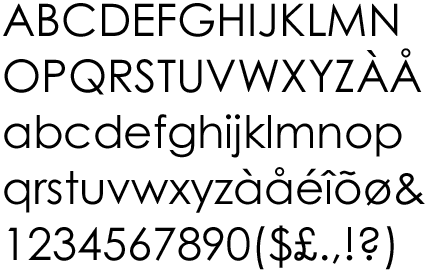
\includegraphics[scale=0.4]{century.png}\caption{Century Gothic, een robuust lettertype dat gebruikt wordt in de leesmethode `Aap-Zee-Koe'.}\label{gothic}
\end{figure}
\noindent Ik heb ook enkele autileerlingen geobserveerd toen ze op de computer 
aan het spelen waren en het viel erg op dat zij, als ze vrij op de computer 
mogen, gefascineerd zijn door foto's van zichzelf en de klasgroep. Ze doen niet 
liever als foto's en filmpjes van de klas telkens opnieuw te herbekijken.

\subsubsection{Logopedie}
Ik heb bij mijn observaties ook een paar keer logopediste Martine gaan bezoeken, 
die vaak leerlingen in kleine groepjes apart neemt om bepaalde vaardigheden te 
ontwikkelen. Zo heb ik een sessie geobserveerd met twee leerlingen met het 
syndroom van Down die suiker en zout moesten proeven om zo het onderscheid 
tussen deze twee smaken aan te leren. Het was erg opvallend hoe zij dit absoluut 
niet konden onderscheiden van elkaar en het allebei erg lekker vonden. Deze twee 
leerlingen maakten ook altijd mopjes onder elkaar (het zout verstoppen,...).
Uiteindelijk is de sessie dan geëindigd door het visuele onderscheid tussen een 
pot suiker en pout zout duidelijk te maken, vermits het via de smaakzintuigen 
niet werkte.\\


\noindent Ook heb ik in een andere sessie een memoryspel gespeeld rond 
groenten, waarbij ze het woord van een groente (bv. bloemkool) moesten linken aan een tekening en een foto van 
een bloemkook. Bedoeling van zo'n oefeningen is hen laten bewust worden dat het 
woord, de tekening en de foto over dezelfde concepten gaan en geen verschillende 
dingen zijn.

\subsection{Algemene conclusies}
Na mijn hele observatieweek kwam ik tot een aantal conclusies:
\begin{itemize}
  \item Het valt op dat de leerkrachten echt de zelfstandigheid bij de 
  leerlingen willen ontwikkelen. Leerlingen worden niet zomaar geholpen (bij het eten, bij de jassen aandoen, bij het kuisen,...), maar 
  worden altijd aangespoord om het zelf te doen als ze het zelf kunnen.
  \item Elke schooldag is een hele logistieke operatie. Maar liefst 24 bussen 
  voeren leerlingen naar de Heemschool vanuit de hele, uitgebreide regio rond de school. 
  Dit komt uiteraard omdat er maar een beperkt aantal scholen zijn voor 
  buitengewoon onderwijs. 
    \item Tijdens gesprekken met de leerkrachten, maar ook tijdens de observaties 
  viel het op dat de ondersteuning van de ouders cruciaal is bij het 
  ontwikkelingsproces. Leerlingen met een beperking die van thuis uit nauwelijks 
  tot niet ondersteund worden, worden meestal nog extra vertraagd in hun 
  ontwikkeling.
  \item Heel veel leerlingen komen uit schrijnende opvoedingssituaties. Sommige 
  leerlingen zijn zelf gedwongen geplaatst op internaat in het Heemhotel en 
  wonen aldus permanent op de Heemschool. Schrijnende opvoedingssituaties die ik geobserveerd heb zijn 
  onder meer kinderen uit gezinnen die onder de armoedegrens leven en aldus sociaal 
  achtergesteld zijn, kinderen die het gevolg zijn van een incestieuze 
  verhouding tussen familieleden en daar hun handicap aan te danken hebben en 
  kinderen waarvan de ouders zelf gehandicapt zijn en de handicap genetisch hebben doorgegeven. 
  \item Op de Heemschool zijn er ook een aantal leerlingen die illegaal in het land verblijven, waardoor zij niet op de mutualiteit kunnen terugvallen om aan hun zorgbehoeften te voldoen.
  Zo zijn er leerlingen die eigenlijk in een aangepaste roelstoel zouden moeten zitten, 
  maar door hun illegaal verblijf hier geen recht op hebben.
  \item Het viel op hoe `respectvol' de leerkrachten met de leerlingen omgaan. 
  Nooit heb ik een leerkracht gezien die zijn geduld verloor en daardoor grof 
  werd ten overstaande van leerlingen. Het clichébeeld van scholen voor andersvaliden 
  waar de leerlingen slecht 
  behandeld worden omdat ze het toch niet zullen kunnen navertellen, klopt helemaal niet.
  \item Hoewel je enorm snel wendt aan het zwakke cognitief ontwikkelingsniveau 
  van de leerlingen, mag je ze toch ook niet onderschatten. Zo weten sommige 
  leerlingen verdomd goed hoe ze je psychologisch moeten bespelen. Ook praten 
  over leerlingen waar de leerling zelf bij is (onder het mom van: hij/zij verstaat het toch niet) 
  is absoluut te mijden: ze weten verdomd goed als het over hen gaat.
  \item Voor mijn informaticaproject viel het mij tijdens de observaties vaak op 
  dat - hoe zwak ze ook presteren op bepaalde vaardigheden zoals lezen en 
  schrijven - ze vaak zeer goed zijn in het spelen van computerspelletjes en het 
  hanteren van de computer in het algemeen. 
  
  
  
\end{itemize}

\newpage
\section{Eigen project}\label{project}
\subsection{Wat vooraf ging}
In mijn motivatiebrief had ik geschreven dat ik graag mijn informaticakennis ten 
dienste van de stageschool wou stellen, en dat ik tijdens de observatie ging rondkijken 
hoe ik dat kon omzetten in een project. Dat resulteerde dan tijdens de observatieweekjes in een oproep op Smartschool (Figuur \ref{oproep}) waarbij de klasleerkrachten ideeën voor oefeningen, spelletjes of kleine programma's konden insturen die 
ze zouden kunnen gebruiken tijdens hun lessen op het aanwezige ICT-materiaal in de school. Ook tijdens mijn observaties hadden sommige leerkrachten reeds ideeën aangereikt. \begin{figure}[h!]
  \centering
  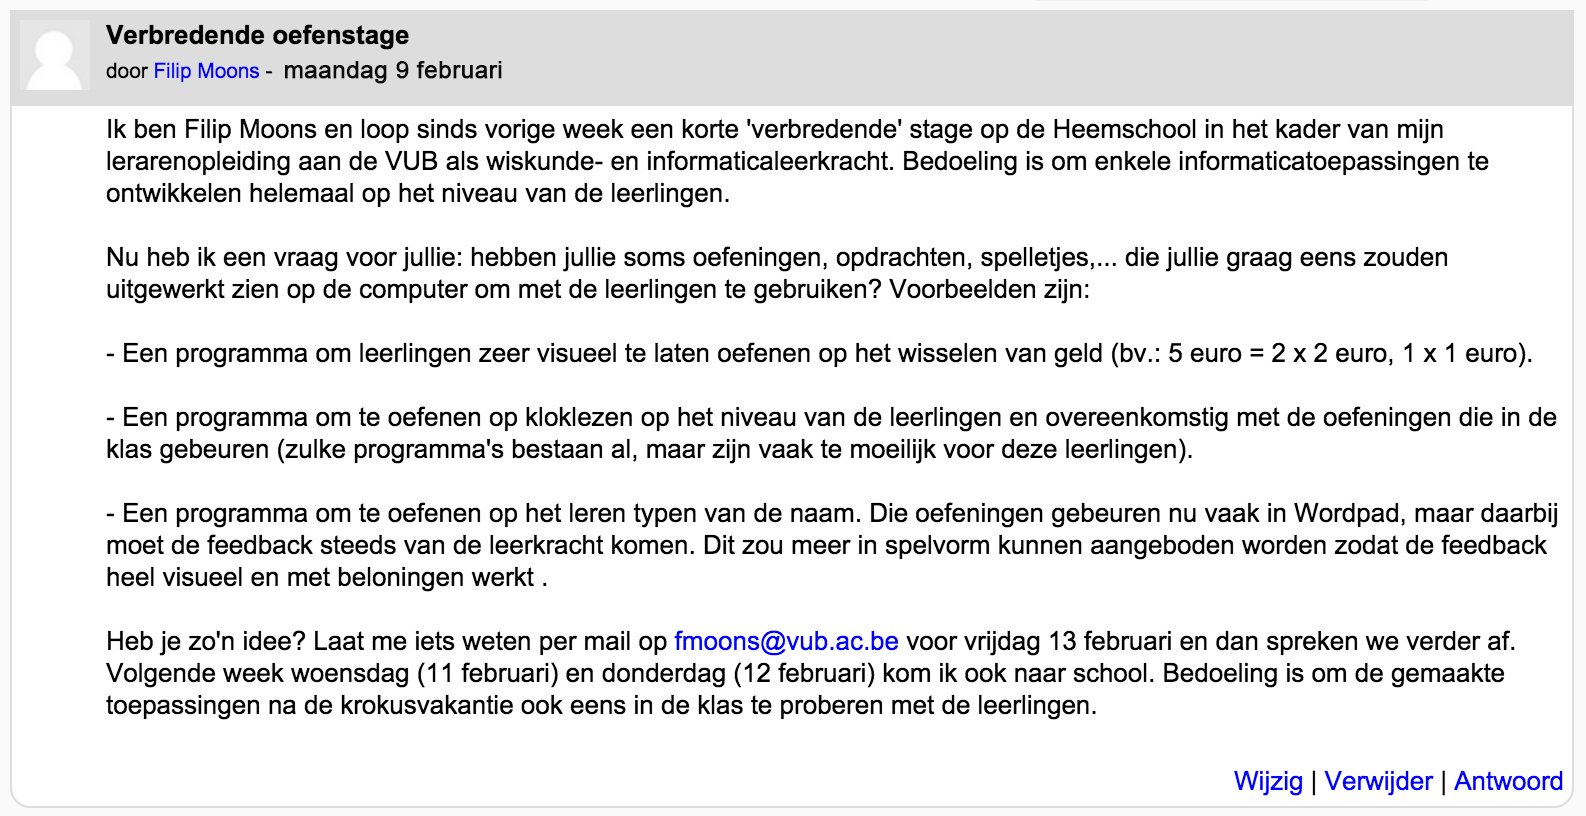
\includegraphics[scale=0.27]{oproep.jpg}\caption{De oproep aan de leerkrachten om ideeën voor ICT-materiaal in te sturen op Smartschool.}\label{oproep}
\end{figure}
\\
 
\noindent Die oproep op Smartschool bleef niet zonder gevolg, want ik heb hierop heel wat reactie gekregen. Heel veel ICT-materiaal bestaat wel voor het reguliere onderwijs, maar dat materiaal is 
vaak al snel te moeilijk voor deze leerlingenpopulatie (te hoge moeilijkheidsgraad, oefeningen met een tijdslimiet die voor deze leerlingen onhaalbaar is,...). Uiteindelijk kwamen de volgende vragen binnen om te ontwikkelen:
\begin{itemize}
\item Oefenprogramma voor de leesmethode aap-zee-koe, een leesmethode voor leerlingen met 
autismespectrumstoornis.
\item Een programma om leerlingen zeer visueel te laten oefenen op het wisselen van geld (bv.: 5 euro = 2 x 2 euro, 1 x 1 euro).
\item Een programma om te oefenen op kloklezen op het niveau van de leerlingen en overeenkomstig met de oefeningen die in de klas gebeuren (zulke programma's bestaan al, maar zijn vaak te moeilijk voor deze leerlingen).
\item Een programma om te oefenen op het tellen tot 20 en dit in verschillende spelvormen.
\item Een programma om prentpuzzels mee op te lossen.
\item Een programma met een dierenspel waar geluiden met de juiste dieren moeten 
verbonden worden.
\end{itemize}
Ik ben uiteindelijk op alle vragen van de leerkrachten kunnen ingaan, geen enkele oproep heb ik moeten afwijzen want alle voorstellen waren haalbaar binnen de tijdspanne van de stage. 
Elke ICT-toepassing kwam tot stand in uitgebreid overleg met de vragende 
leerkrachten. Nadien is ook elk programma getest geweest met de klas of met 
individuele leerlingen. Hoe elk projectje tot stand kwam en wat het resultaat 
van die testen waren, leg ik toepassing per toepassing uit in de volgende sectie. In 
de uitleg ga ik wel niet dieper in op de technische en technologische aspecten van de ICT-toepassingen, 
vermits ik veronderstel dat de lezers van dit verslag hier geen voorkennis over 
hebben.\\

\noindent\framebox(440, 40){ 
\parbox{430\unitlength}{De lezer die niet kan wachten op de sectie eindresultaat om het gemaakte ICT-materiaal te proberen, kan nu al surfen
naar \textbf{www.filipmoons.com/heemschool} om alle oefeningen uit te testen.}
}
\subsection{De ICT-toepassingen}
\subsubsection{Tellen tot 20 - Klas van Elke Janssens (Heemklas 2)}
In de Heemklas 2 (leeftijd tussen 6 en 9 jaar) leren de leerlingen tellen tot 20. De klasleerkracht Elke 
Janssens heeft daarbij allerlei oefeningen gevonden op de computer voor te 
oefenen op tellen tot 10 (o.a. op \textt{http://www.hethofderspelen.nl/}), maar zo goed als alle oefeningen met hogere getallen worden dan gecombineerd met optellen en vermenigvuldigen. 
De vraag kwam er dan ook oefeningen te ontwikkelen waarbij louter de vaardigheden  
rond tellen tot 20 getest worden. Uiteindelijk heb ik, in samenspraak met Elke, 
volgende oefeningen ontwikkeld:
\begin{figure}[h!]
        \centering
        \begin{subfigure}{.5\textwidth}
          \centering
                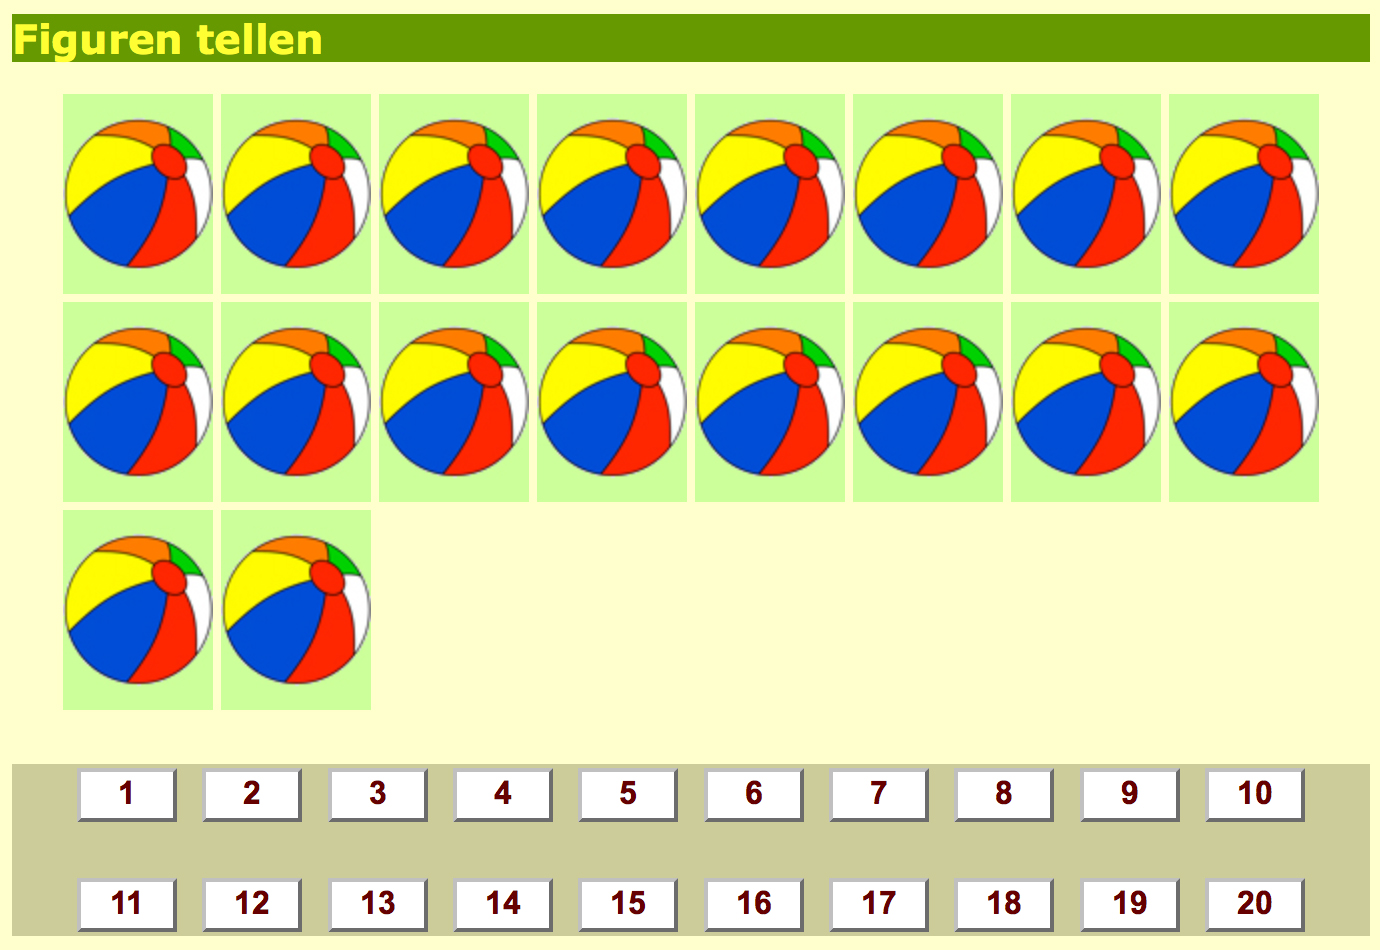
\includegraphics[scale=0.15]{20_1.jpg}
                \caption{Figuren tellen.}
                \label{20_1}
        \end{subfigure}%
        \begin{subfigure}{.5\textwidth}
           \centering
                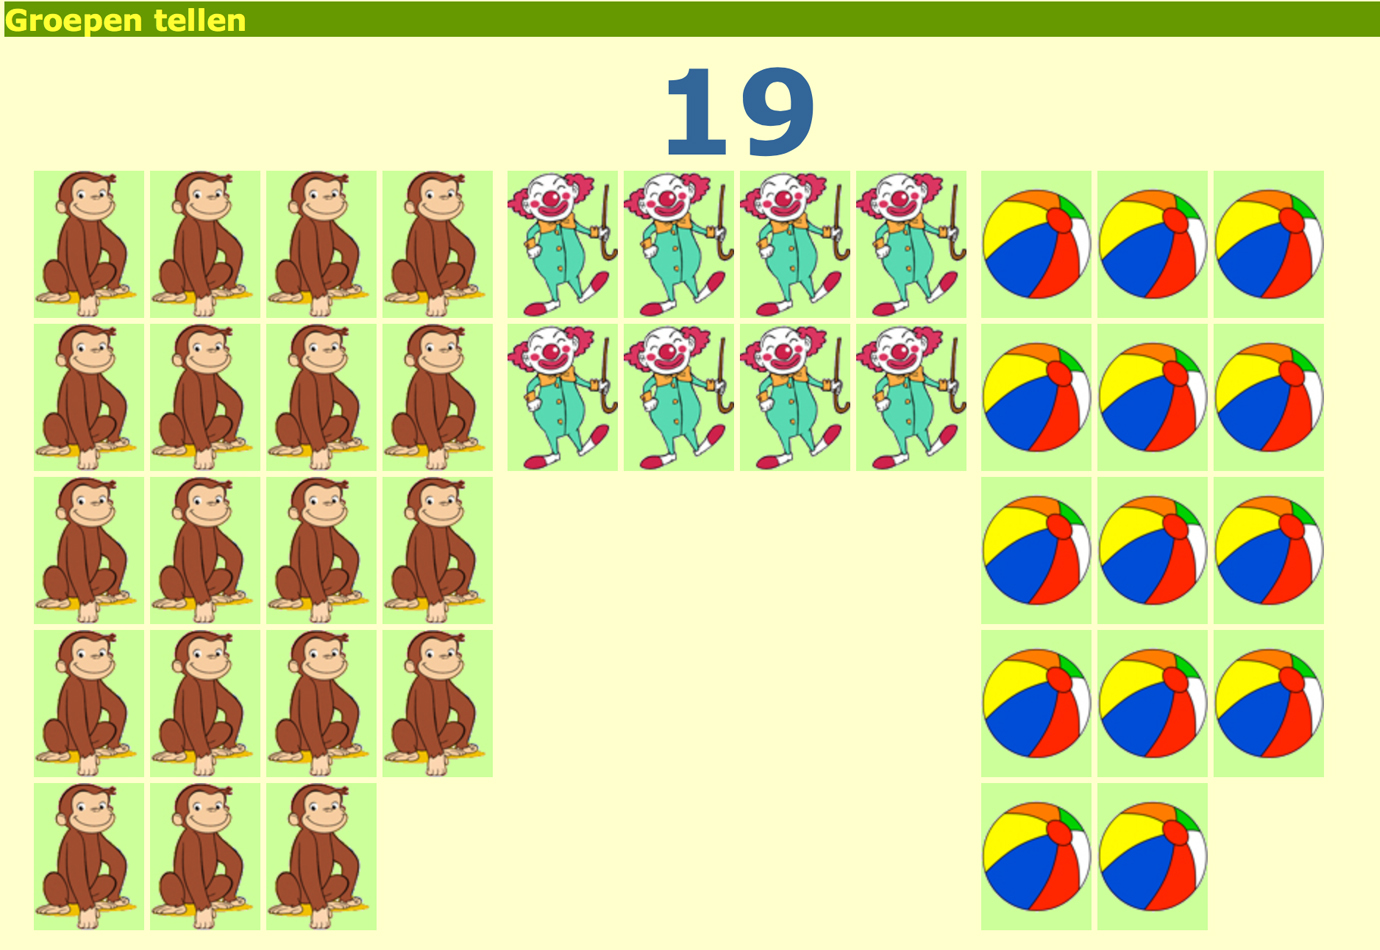
\includegraphics[scale=0.15]{20_2.jpg}
                \caption{Groepen tellen.}
                \label{20_2}
        \end{subfigure}
     
          \begin{subfigure}{.5\textwidth}
          \centering
                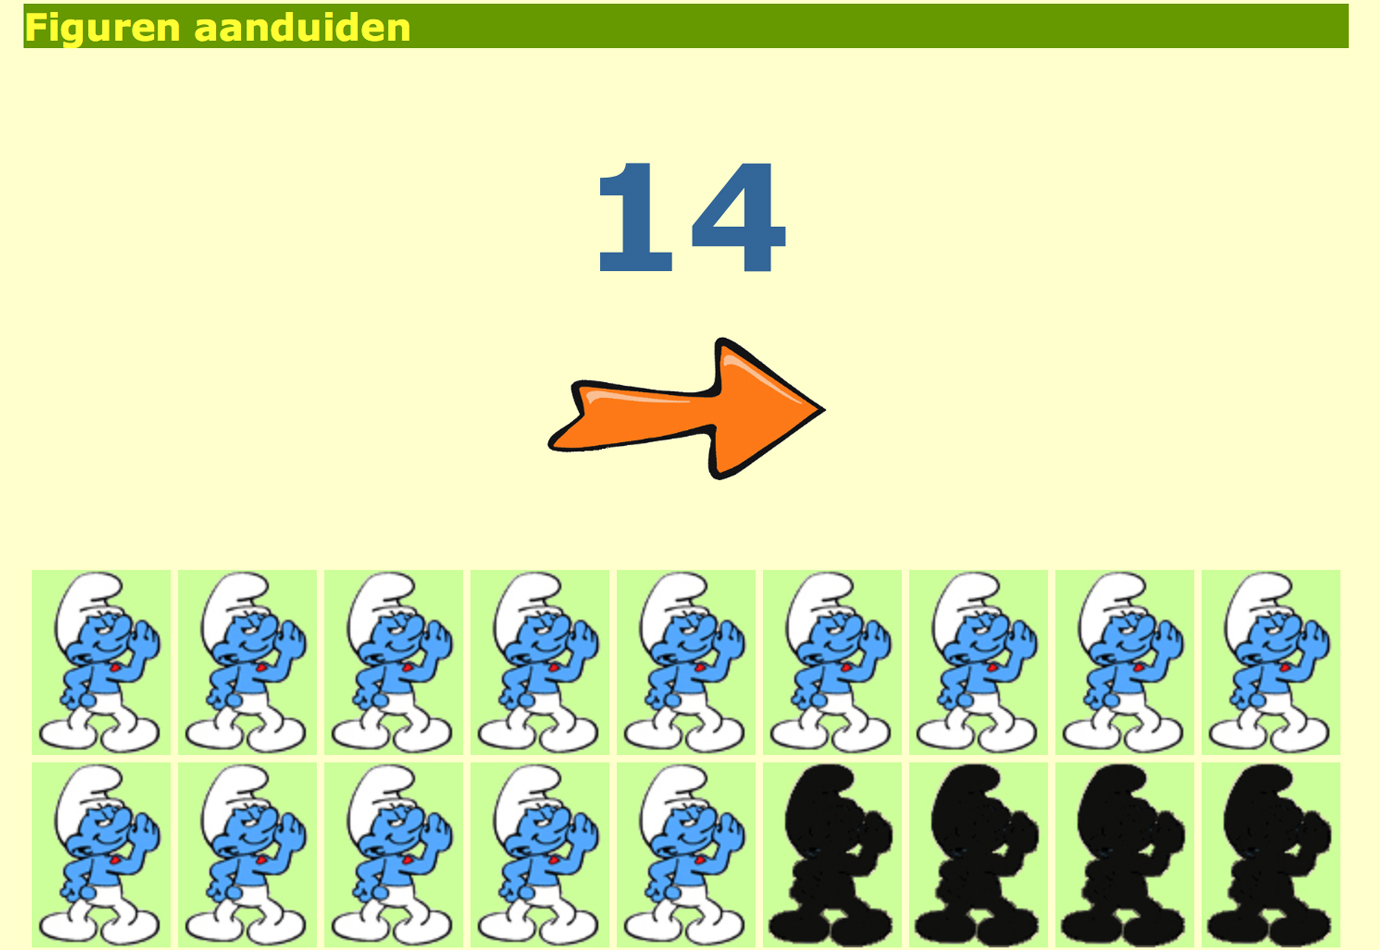
\includegraphics[scale=0.15]{20_3.jpg}
                \caption{Figuren aanklikken tot een gegeven getal.}
                \label{20_3}
        \end{subfigure}%
        \begin{subfigure}{.5\textwidth}
           \centering
                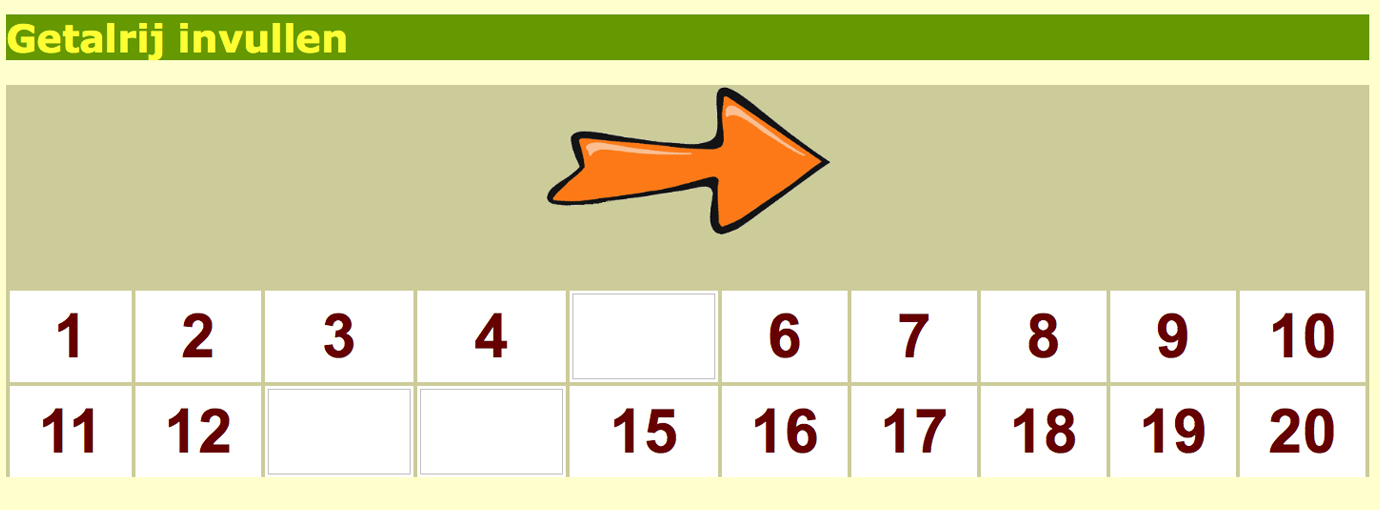
\includegraphics[scale=0.15]{20_4.jpg}
                \caption{Getalenrij aanvullen.}
                \label{20_4}
        \end{subfigure}        \caption{Screenshots van oefeningen rond tellen tot 
        20.}.
\end{figure}

\begin{itemize}
  \item Een oefening waarbij een willekeurig aantal figuren verschijnt (tot 20) 
  en ze moeten aangeven hoeveel figuren er weergeven worden. (Figuur 
  \ref{20_1} is hiervan een screenshot).
  \item Een oefening waarbij er een willekeurig getal verschijnt (tot 20) en verschillende 
  groepen van figuren. Ze moeten de groep aanklikken die hetzelfde aantal 
  figuren heeft als het gegeven getal. (Figuur \ref{20_2} is hiervan een screenshot)
  \item Een oefening waarbij er een getal verschijnt (tot 20) en ze net evenveel figuren moeten aanduiden als dat getal (screenshot in Figuur \ref{20_3}).
  \item Een oefening waarbij de getallenrij tot 20 wordt weergeven met telkens 3 
  willekeurige getallen weggelaten. Zij moeten de weggelaten getallen dan aanvullen (Figuur 
  \ref{20_4}).
\end{itemize}

\noindent Bij deze oefeningen is het belangrijk om te weten dat de leerlingen niet kunnen 
lezen en dat bijgevolg alle opdrachten moeten voorgelezen worden en feedback ook 
enkel via spraak en/of geluid kan. Hiervoor heb ik steeds beroep gedaan op een vriend 
met een heldere stem om al deze zaken in te spreken, omdat ik het persoonlijk te 
confronterend vind om steeds met mijn eigen stem geconfronteerd te worden als ik 
de oefeningen test met leerlingen. \\

\noindent Uiteindelijk werden de oefeningen gezamenlijk getest met alle 
leerlingen van de klas in het computerlokaaltje. Ook stagebegeleidster Evelyne De Smet was bij dit testmoment aanwezig.
 Ze bleken hier heel goed mee weg te kunnen, al vonden ze de oefening met de 
 getallenrij wel zeer moeilijk. Er bleek wel in de testfase nog een foutje in de 
 oefening van de getallenrij te zitten, want om de oefening te doen moet je gewoon naar mijn website surfen, 
maar daar vult de webbrowser automatisch vorige antwoorden aan bij tekstvakken. 
Dit heb ik uitgeschakeld in de finale versie.

\subsubsection{Kloklezen \& Geld wisselen - Klas van Anne-Marie (Heemklas 3)}
In de Heemklas 3 (leeftijd tussen 9 en 11 jaar) bij Anne-Marie leren de leerlingen 
voornamelijk socialiseren: zo leren ze de klok lezen en naar de winkel gaan. In 
dat kader vroeg Anne-Marie mij een aantal oefeningen te ontwikkelen rond 
kloklezen en geld wisselen.\\

\paragraph{Kloklezen}
\noindent Bij het kloklezen is de moeilijkheid bij bestaande computeroefeningen vaak dat 
ze veel te moeilijk zijn voor deze doelgroep. Zo leren de leerlingen hier in eerste instantie per 
kwartier de klok aflezen (kwart voor 4, kwart over 4, half 5, kwart voor 5) en 
pas dan per vijf minuten (bv. 12:55). Ook de klok is in het leerproces heel specifiek  
van vorm: de kleine wijzer heeft een blauwe kleur, de grote wijzer een rode. In 
eerste instantie heb ik rond klok lezen twee oefeningen ontwikkeld:
\begin{itemize}
  \item Een oefening waarbij ze een willekeurig gekozen tijdstip per kwartier moesten aanduiden op 
  de klok. Ze krijgen bijvoorbeeld `kwart over vijf' als opgave en moeten dan 
 de wijzers juist zetten op de klok. De grote, rode wijzer is zo ingesteld dat 
 hij enkel per kwartier kan gezet worden. (Figuur \ref{klok1}).
 \item Een oefening waarbij ze het willekeurig gekozen tijdstip per kwartier moesten aflezen van de 
 klok. Zo toonde de klok bijvoorbeeld het tijdstip 6:30 en moeten zij intypen 
 `half 7'. (Figuur \ref{klok2})
\end{itemize}
\begin{figure}[h!]
        \centering
        \begin{subfigure}{.5\textwidth}
          \centering
                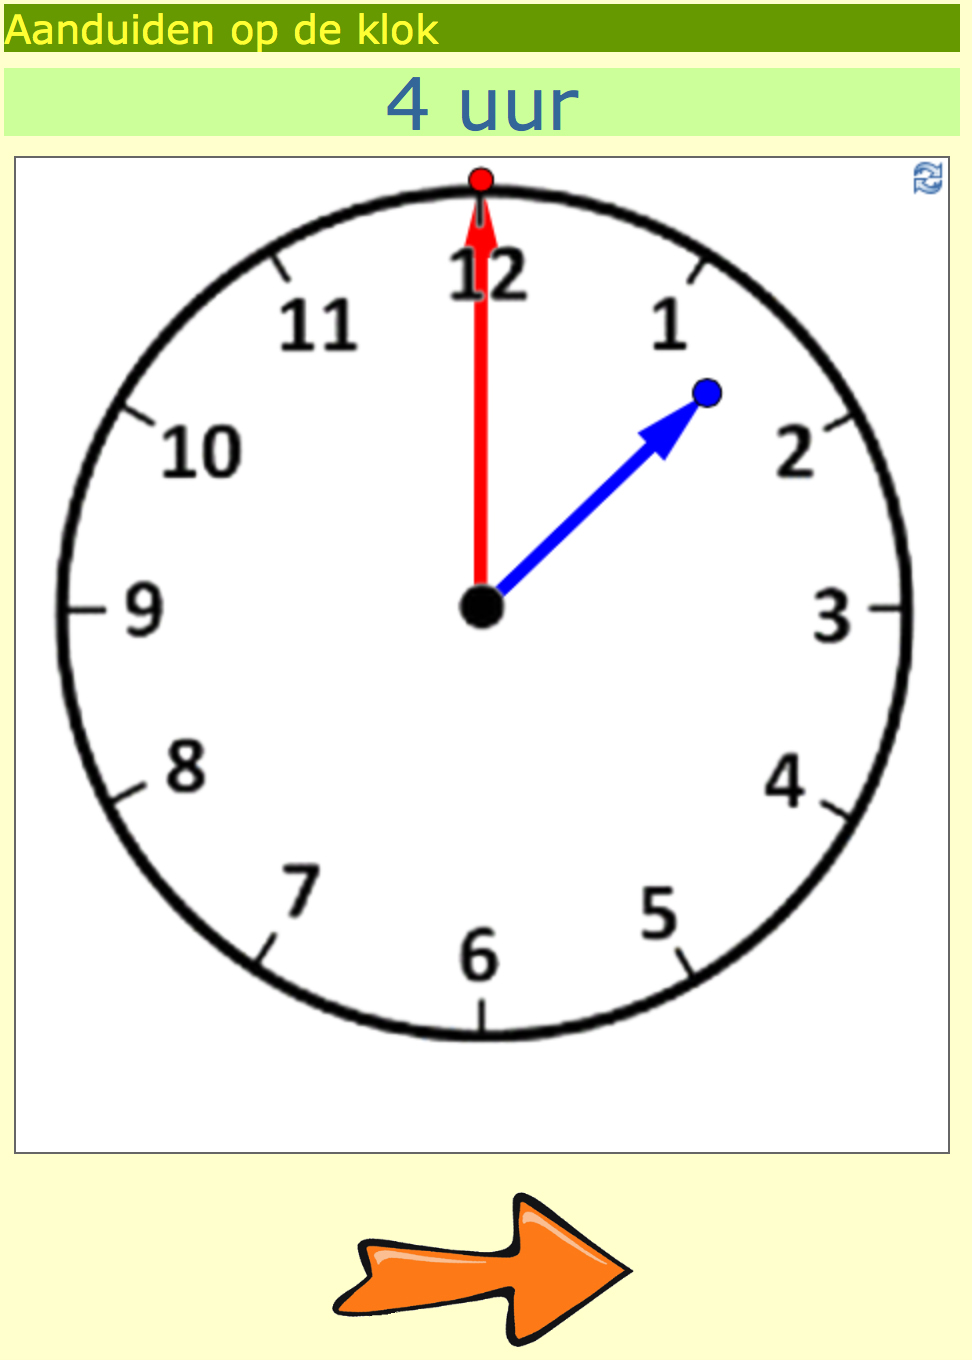
\includegraphics[scale=0.15]{klok1.jpg}
                \caption{Uur aanduiden op de klok.}
                \label{klok1}
        \end{subfigure}%
        \begin{subfigure}{.5\textwidth}
           \centering
                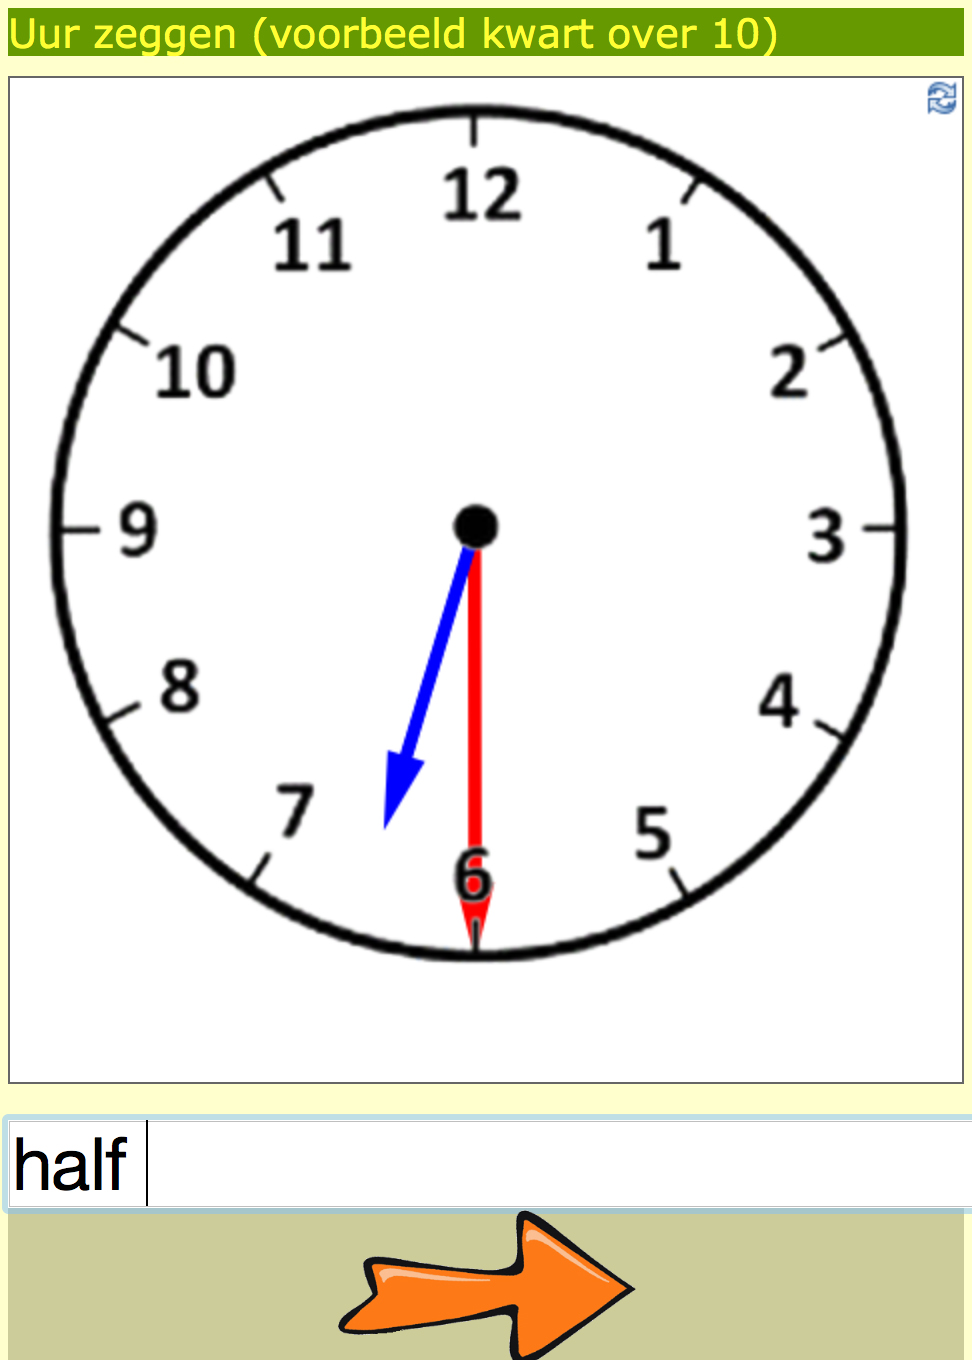
\includegraphics[scale=0.15]{klok2.jpg}
                \caption{Uur aflezen van de klok.}
                \label{klok2}
        \end{subfigure}
           \caption{Screenshots van oefeningen rond kloklezen.}
\end{figure}

\noindent Bij het ontwikkelen heb ik rekening gehouden met de specifieke noden 
van deze doelgroep zoals het respecteren van de kleuren van de wijzers. Zij 
kunnen al beperkt lezen, dus een uur schriftelijk tonen op het scherm dat zij op 
een klok moeten aanduiden zou in principe geen probleem mogen zijn. Om niet 
teveel prikkels tegelijkertijd op de leerlingen af te sturen en ook omdat de leesvaardigheid van de leerlingen toch niet volledig ontwikkeld is, worden de 
opdrachten en de feedback wel via spraak \& geluid doorgegeven. Opnieuw werden deze opdrachten ingesproken door mijn vriend. Deze leerlingen 
kunnen goed met de muis overweg, waardoor het aanwijzen van de wijzers van de 
klok normaal rechtstreeks door het klikken op de wijzers kan gebeuren en er hier 
geen extra's (zoals werken met makkelijker hanteerbare schuifbalken) moeten voorzien worden. 
Ook het typen zou normaal voldoende ontwikkeld moeten zijn om zaken zoals `kwart 
voor 6' in te geven.\\
 
\noindent De oefeningen rond kloklezen werden gezamenlijk getest met de hele klas in het 
computerlokaaltje, simultaan met de oefeningen rond geld wisselen. Ook stagebegeleidster Evelyne De Smet was bij dit testmoment aanwezig. 
Het kloklezen ging eigenlijk erg goed en de leerlingen konden erg vlot de muis 
hanteren om de wijzers van de klok juist te zetten. Tijdens de testfase waren 
bewust enkel de oefeningen per kwartier ontwikkeld. Wegens het erg enthousiaste 
onthaal van de oefeningen door de klas werden er op vraag van de klasleerkracht Anne-Marie na de testfase dezelfde oefeningen ontwikkeld 
maar nu per 5 minuten. Deze oefeningen zijn identiek aan deze per kwartier, maar de uren worden 
hier onder de `digitale' vorm \texttt{uu:mm} weergegeven, dus bv. 08:50. Zo 
moeten de leerlingen dit ook intypen.

\paragraph{Geld wisselen} Klasleerkracht Anne-Marie wou graag een ICT-oefening 
laten ontwikkelen waarbij een bepaald rond bedrag tot 5 euro (dus 1, 2, 3 en 4 euro) verschijnt en de leerlingen dit op alle mogelijke manieren kunnen
wisselen in stukken van 2 euro en 1 euro. Voor de sterkeren zou er ook eventueel 
50 cent kunnen aan toegevoegd worden. Dit resulteerde in:
\begin{itemize}
  \item Een oefening waarbij een rond bedrag tot 5 euro wordt weergegeven en uitgesproken
  dat zij op een willekeurige manier kunnen wisselen in 2 euro, 1 euro en 50 
  cent. De leerlingen die 50 cent nog niet kennen, kunnen het in eerste 
  instantie negeren en er nadien alsnog mee experimenteren. Een screenshot vind 
  je in Figuur \ref{geld}.
  \end{itemize}
\begin{figure}[h!]
  \centering
  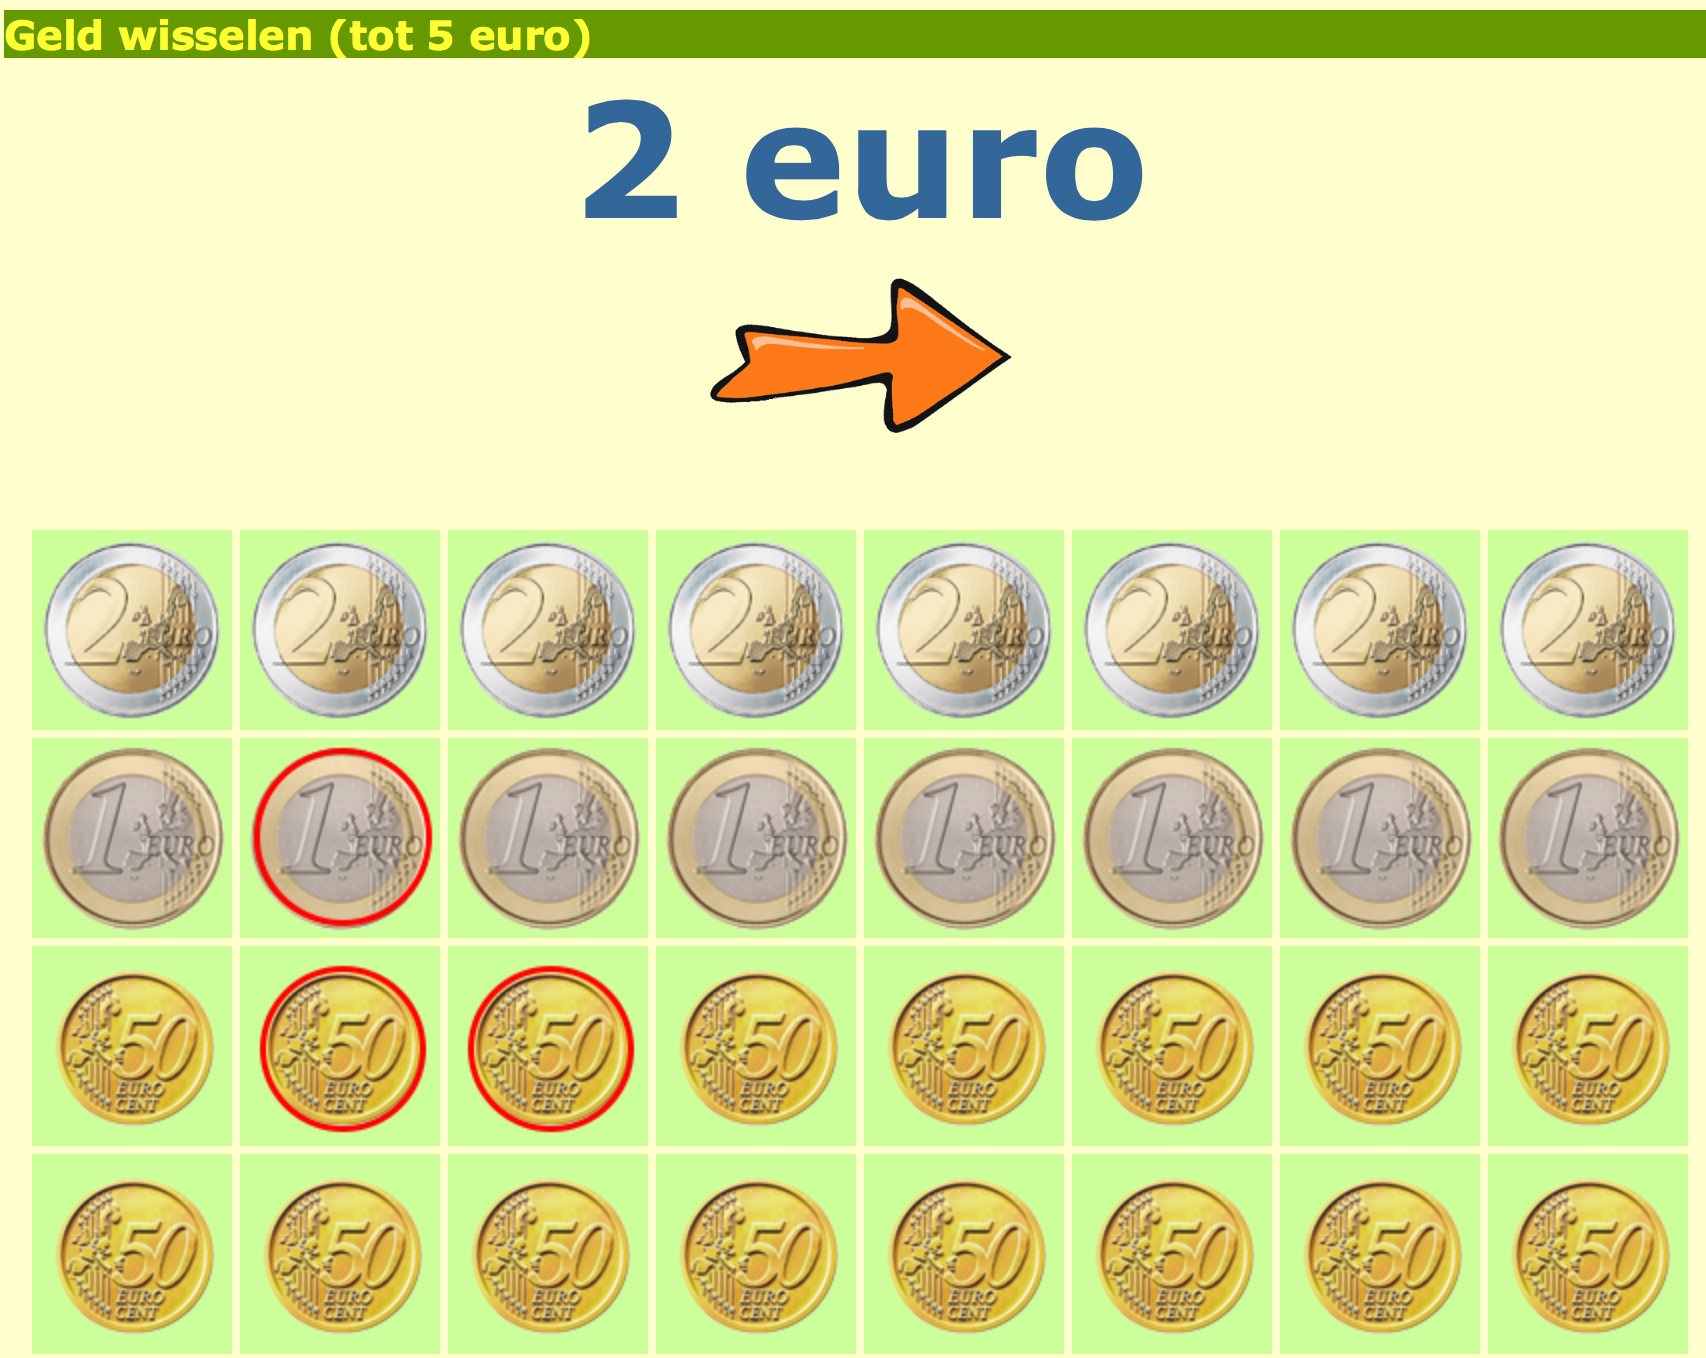
\includegraphics[scale=0.15]{geld.jpg}\caption{Screenshot van een oefening rond geld wisselen.}\label{geld}
\end{figure}

\noindent Bij de ontwikkeling van de `geld wisselaar' heb ik opnieuw rekening 
moeten houden met de beperkte leesvaardigheid van de leerlingen en daarom wordt 
het bedrag zowel neergeschreven weergegeven maar ook via spraak voorgelezen. 
Opnieuw deed ik hiervoor beroep op mijn vriend om alle bedragen in te spreken. \\

\noindent Het testmoment vond samen met het testmoment van de oefeningen rond kloklezen 
plaats en hierbij was ook stagebegeleidster Evelyn De Smet aanwezig. Deze 
oefening werd ook enorm positief onthaald, waardoor er na de testfase ook een 
versie van de oefening is vrijgegeven waarbij geld gewisseld wordt tot 10 euro. 
Hierbij kunnen leerlingen dan kiezen tussen briefjes van 5 euro en muntstukken 
van 2 euro, 1 euro \& 50 cent.



\subsubsection{Leesmethode `Aap-Zee-Koe' - Klas van Liljan (Autiklas)}
Leesmethode `Aap-Zee-Koe' is een leesmethode ontwikkeld door de vereniging 
Autisme Centraal. In de autiklasjes van de heemschool leren ze hiermee de 
sterkere leerlingen lezen. De leesmethode wordt uitgebreider toegelicht bij de observaties onder sectie \ref{auti}. Het grote verschil met een reguliere leesmethode is de veel minder abstracte woordenschat (reguliere leesmethodes gebruiken vaak verhalen die voor sterk
autistische leerlingen te moeilijk zijn om te vatten, zij moeten concrete, letterlijke waarneembare woorden aangeleerd krijgen), 
ze gebruiken in de leesmethode ook een andere robuuster lettertype (Century Gothich, zie Figuur \ref{gothic}) waarin er niet teveel 
tirlantijntjes waardoor de autileerlingen niet afgeleid kunnen worden door de 
details van de letters maar de letters globaal leren onderscheiden. Uiteindelijk 
maakte ik op vraag van leerkracht Liljan volgende oefeningen:

\begin{itemize}
  \item Een oefening waarbij willekeurige foto's van geleerde woorden (bv. een aap, de zee, een pop,...) verschijnen 
  en ze het woordje moeten intypen (Figuur \ref{aap1}).
  \item Een oefening waarbij ze woordjes met de foto's moesten verbinden (Figuur \ref{aap2}). 
 \end{itemize}
 \begin{figure}[h!]
        \centering
        \begin{subfigure}{.5\textwidth}
          \centering
                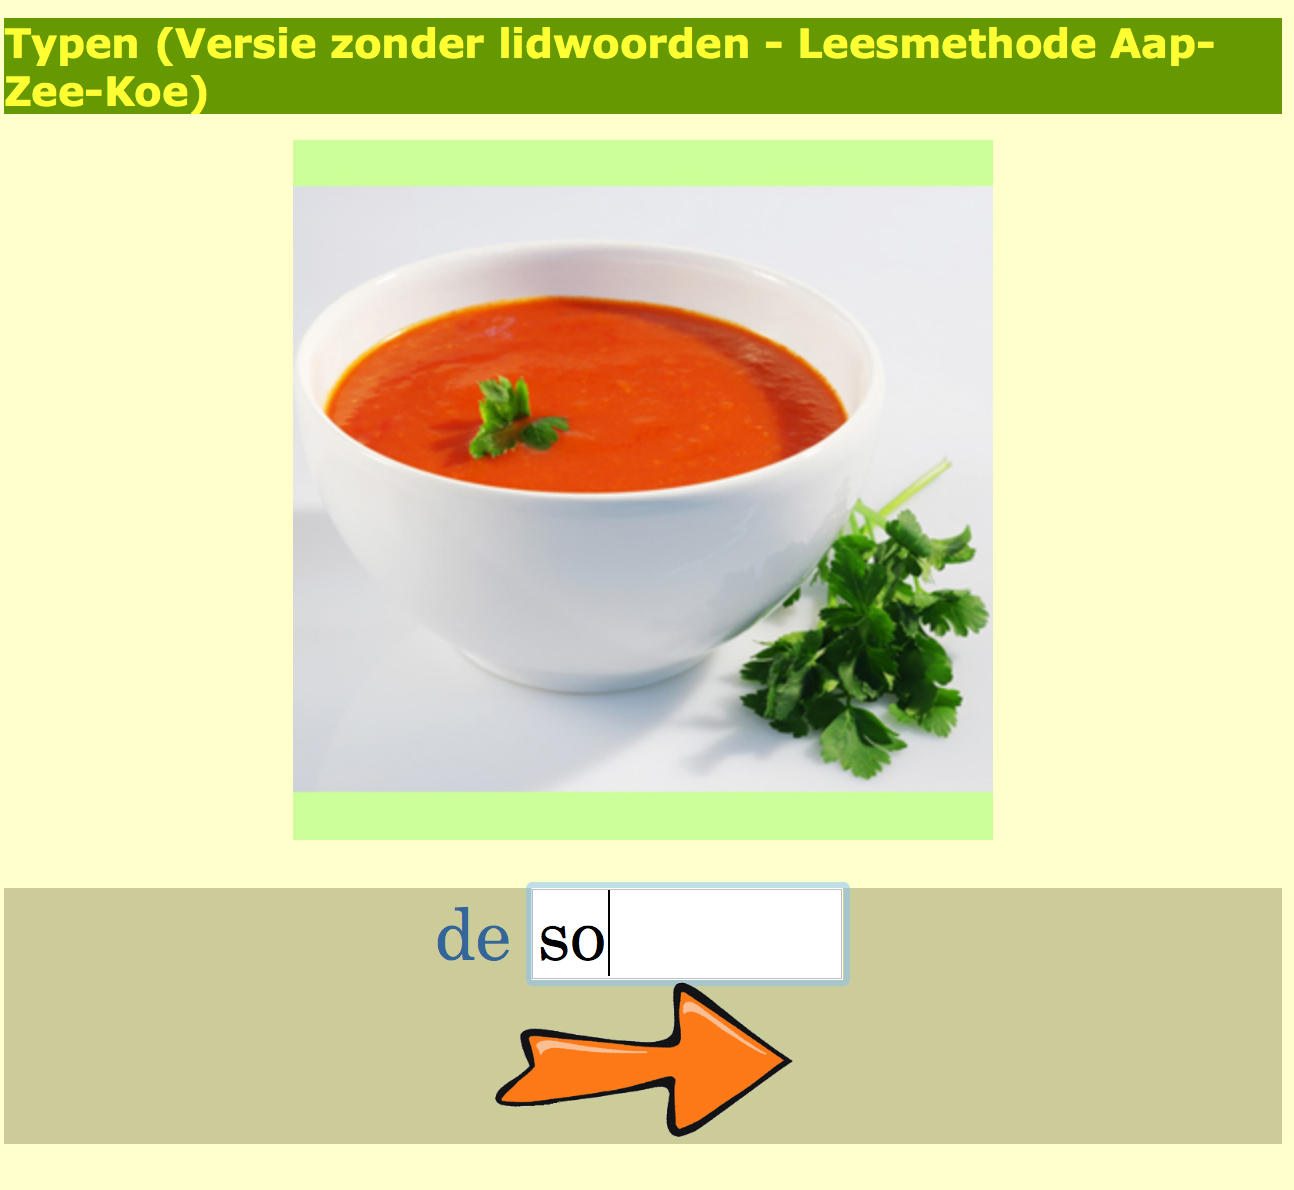
\includegraphics[scale=0.15]{aap1.jpg}
                \caption{Geleerde woordjes intypen.}
                \label{aap1}
        \end{subfigure}%
        \begin{subfigure}{.5\textwidth}
           \centering
                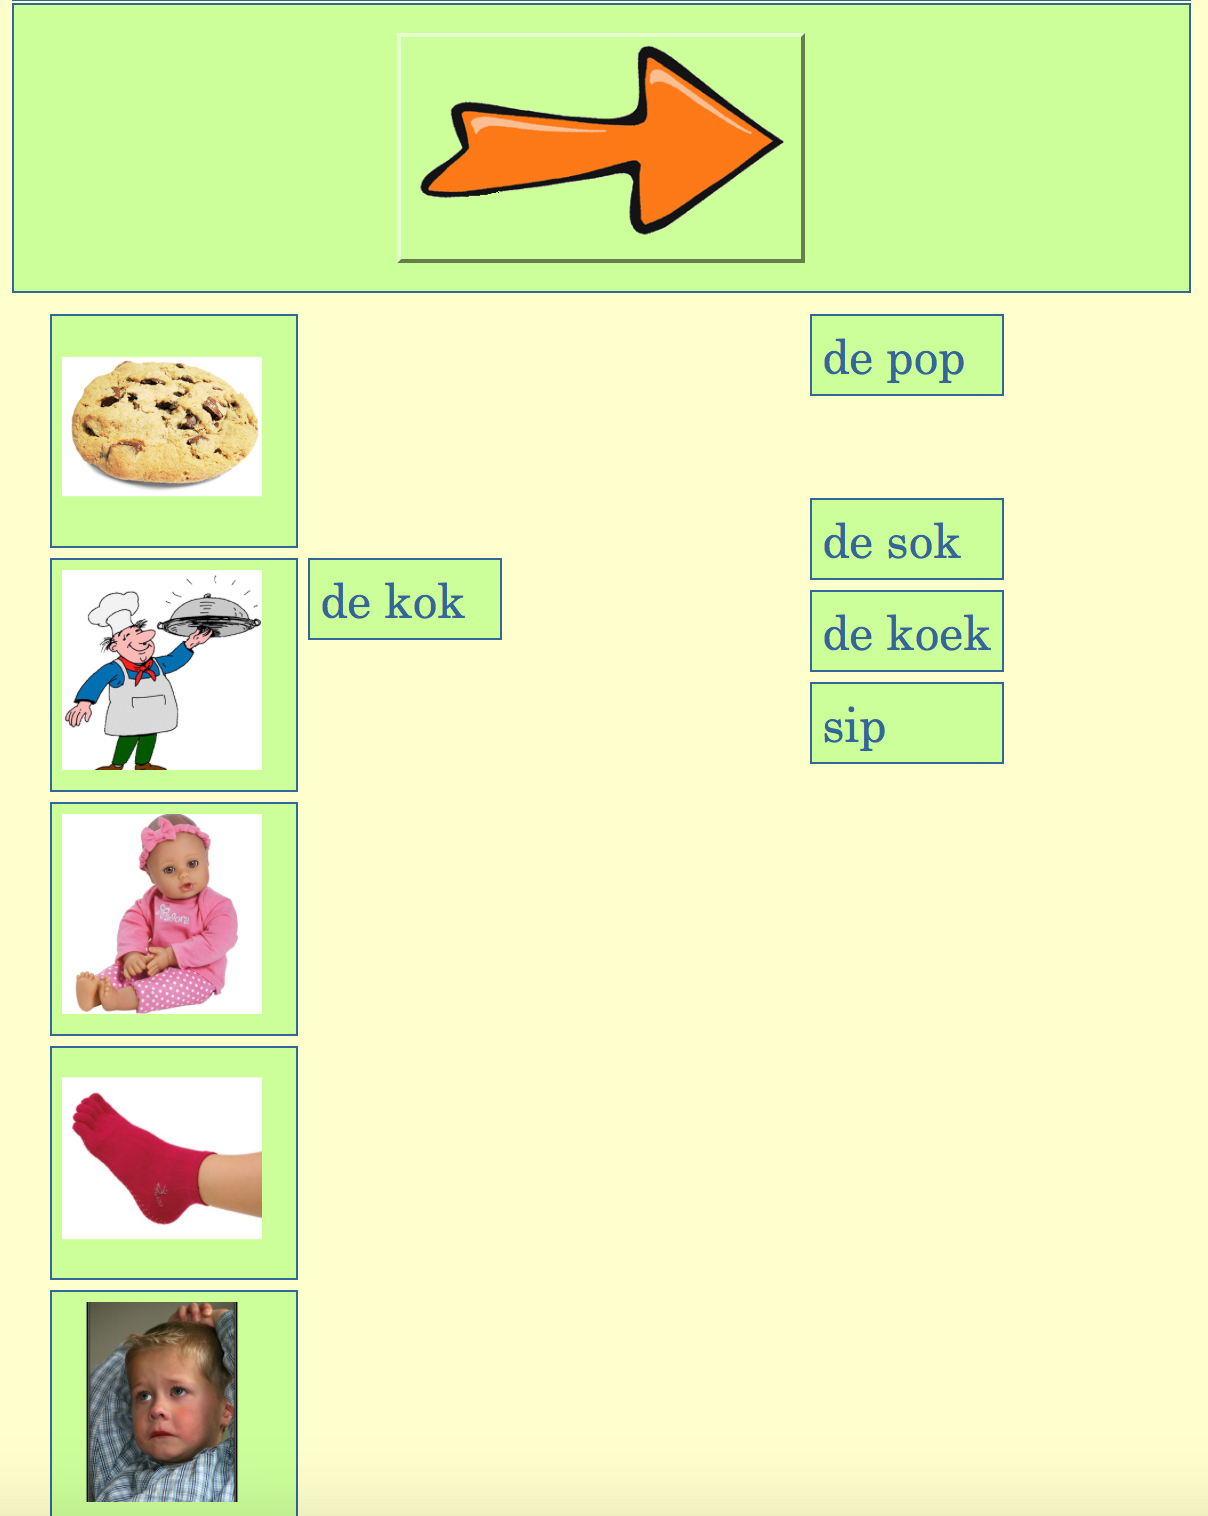
\includegraphics[scale=0.15]{aap2.jpg}
                \caption{Woorden verbinden met de juiste foto.}
                \label{aap2}
        \end{subfigure}
           \caption{Screenshots van de oefeningen rond de leesmethode `Aap-Zee-Koe'.}
\end{figure}
 \noindent Bij de ontwikkeling moest ik er rekening mee houden dat alle woorden in het gebruikte lettertype (Century Gothic) van de 
 leesmethode moesten worden weergegeven en dat alle opdrachten/feedback via spraak 
 \& geluid moesten doorgegeven worden omdat de leerlingen enkel nog maar de 
 aangeleerde woordjes kunnen lezen. Opnieuw heeft mijn vriend alles ingesproken. 
 \\
 
 \noindent Het testen is gebeurd in een groepje van 2 leerlingen. 
 De leerkracht en ik hadden schrik dat er misschien wat moeilijkheden gingen ontstaan met het toetsenbord,
 waarop overal ter wereld de letters in hoofdletters zijn afgedrukt in het lettertype Arial en dit dus afwijkt van het gebruikte lettertype Century Gothic.
 Het idee was om een toetsenbord te maken en de letters te overplakken in het juiste lettertype met etiketten, maar dat bleek niet nodig. Beide leerlingen
 konden zonder veel moeite het verband tussen de lettertypes zien. Een verband dat ze trouwens later in hun ontwikkeling sowieso zouden moeten leren leggen.
    Een leerling 
 was echt razend enthousiast en bleef maar woordjes intypen. Hij had soms wat hulp nodig met het vinden van een letter op het toetsenbord, maar als je één keer de letter aanwees, was hij er de volgende keer mee weg. Ergens was het ook schattig om te zien hoe hij telkens begon te fladderen
 als er positieve feedback door de computer werd gegeven. Een foto genomen door juf Liljan van dit testmoment vind je in Figuur \ref{ferre}. De andere leerling 
 was iets minder vrolijk, maar na overleg met de leerkracht bleek dit algemeen zo te zijn. 
 Na een half uurtje testen, heb ik met de leerlingen nog allerlei foto's genomen 
 met de webcam van mijn laptop
 en hierop allerlei knotsgekke effecten op toegepast. Op één of andere manier 
 zijn zij geweldig aangetrokken tot foto's van zichzelf, want ook bij het 
 observeren viel het me op dat ze niets liever doen dan op de computer foto's van zichzelf en de 
 klas bekijken.

 \begin{figure}[h!]
  \centering
  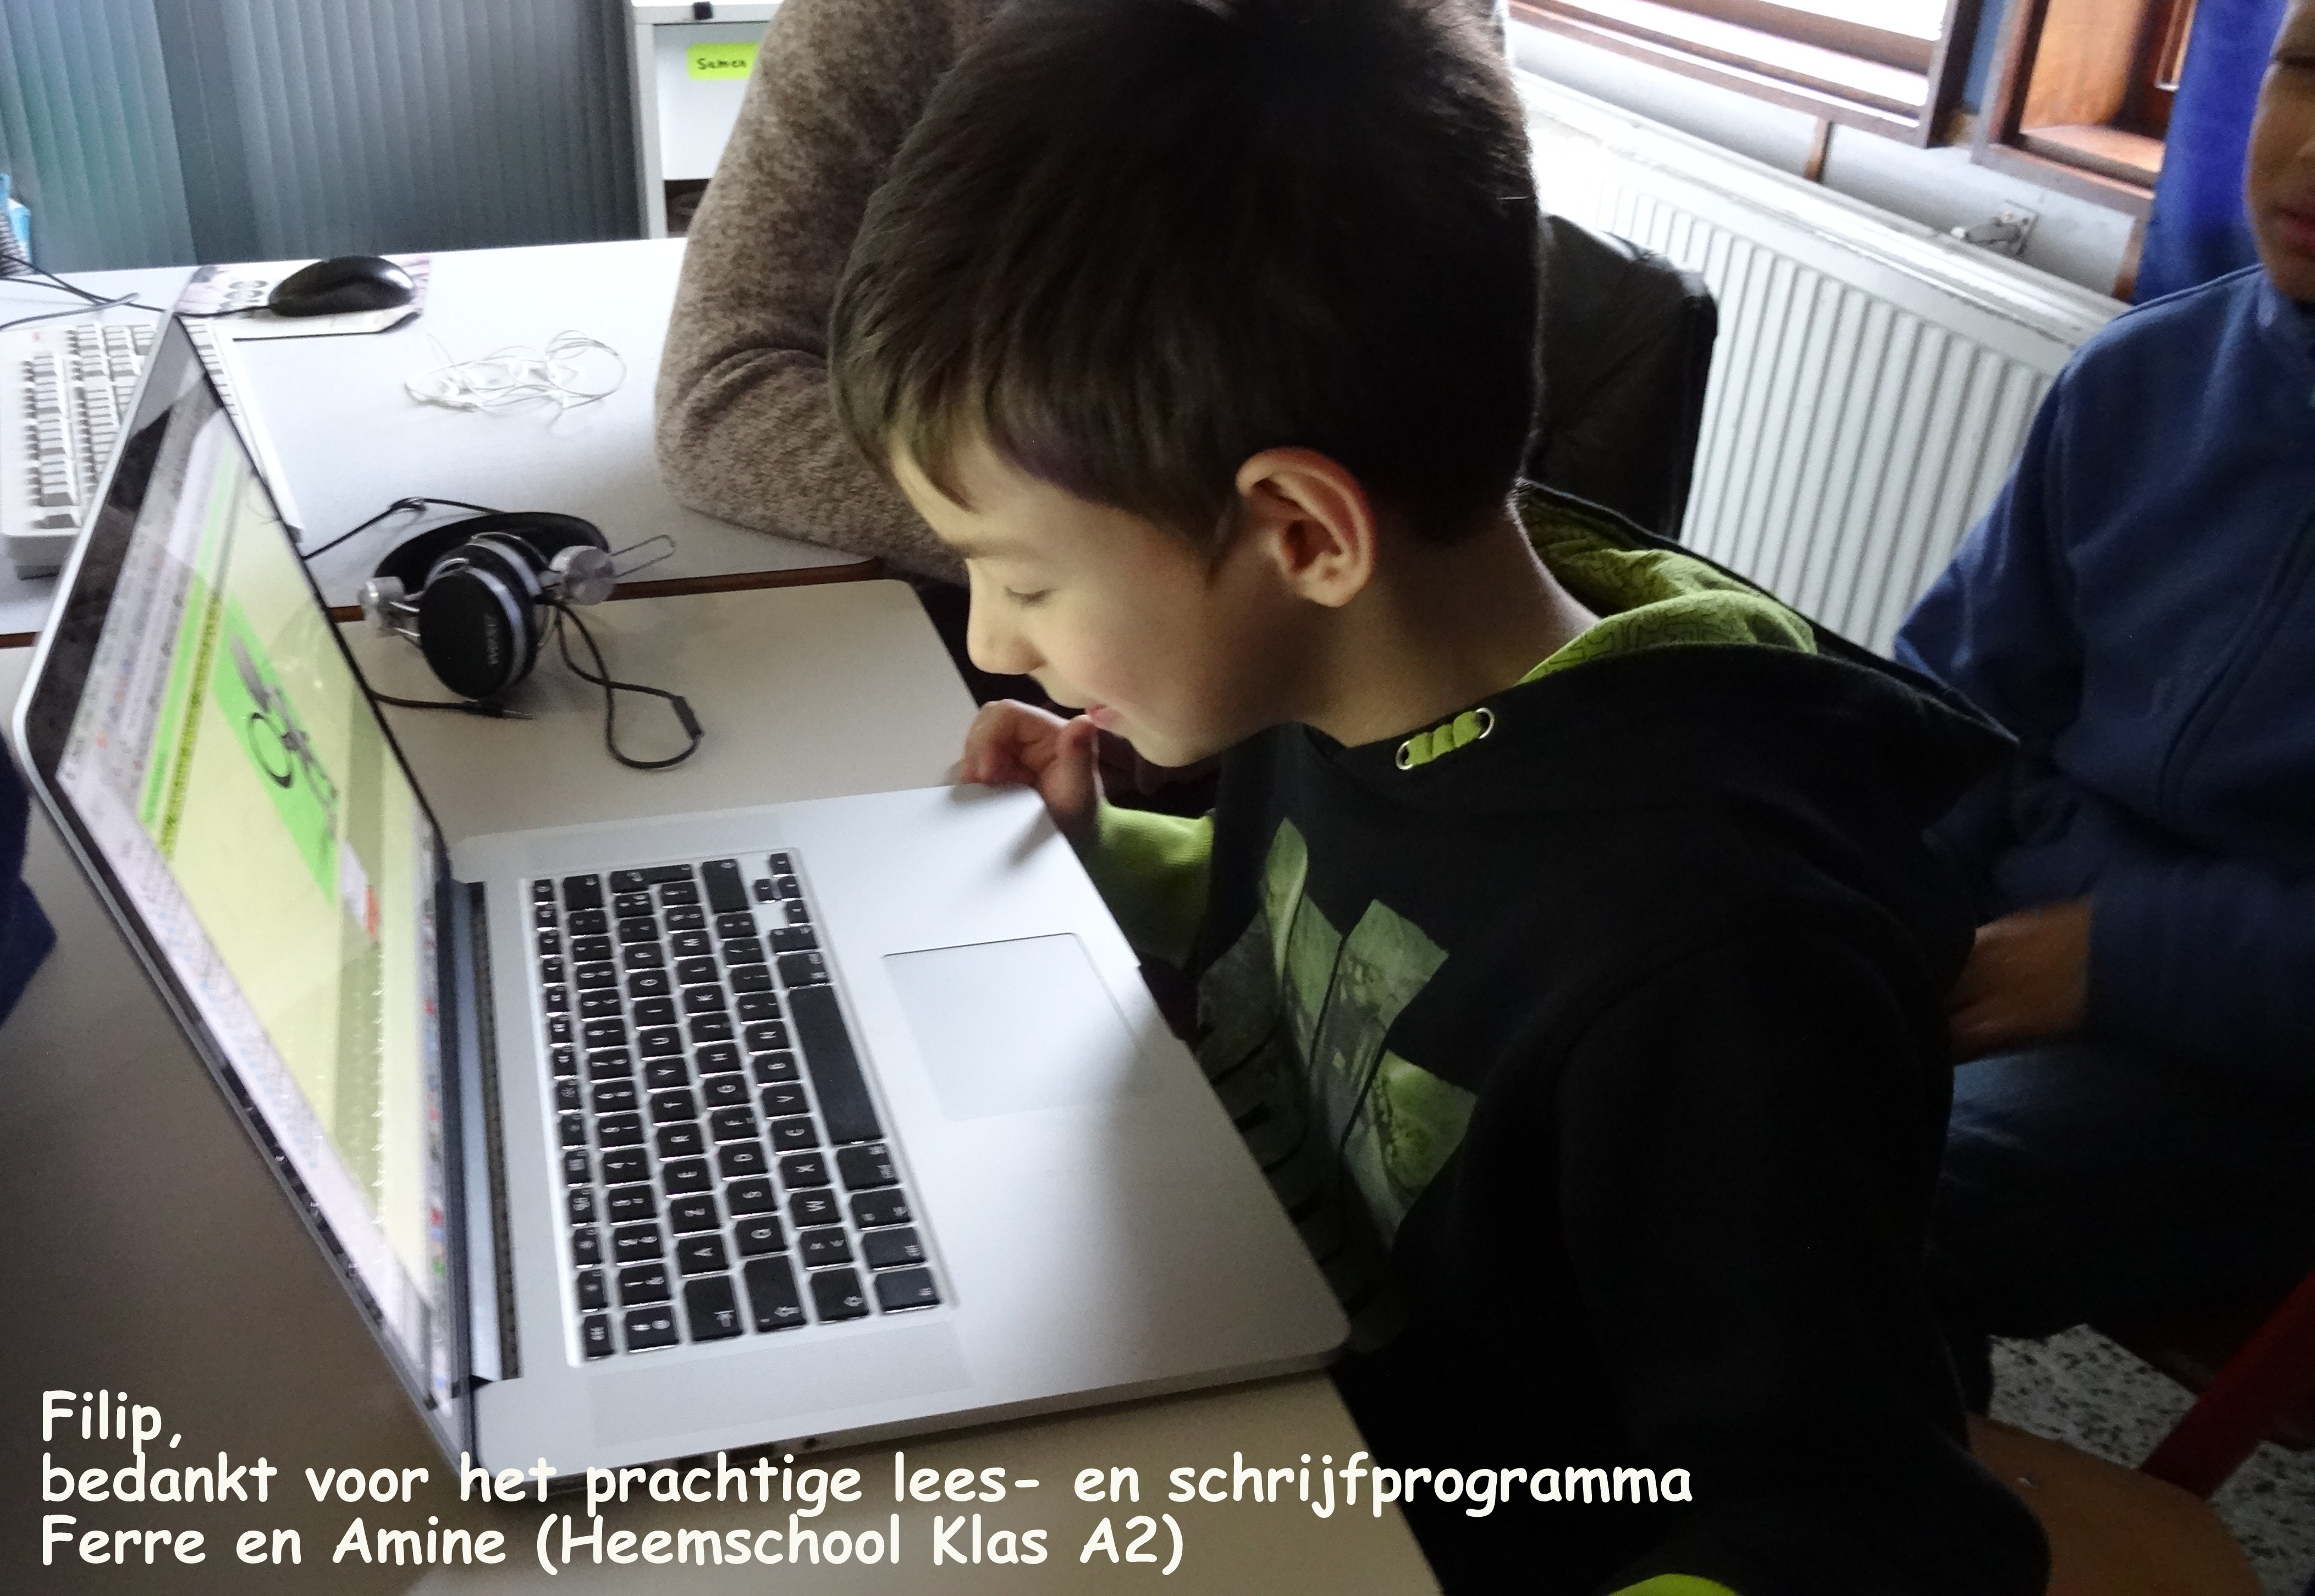
\includegraphics[scale=0.075]{ferre.jpg}\caption{Ferre test het schrijfprogramma uit (Foto van juf Liljan).}\label{ferre}
\end{figure}

\subsubsection{Puzzels \& Dierenspel - Klas van Elke Van Hout (Oriëntatieklas 1)}
De klas van Elke Van Hout is een oriëntatieklasje waarin vooral 
ervaringsgerichte activiteiten centraal staan. Ze vroeg mij dan ook een puzzel 
te maken rond Studio 100-figuren en een dierenspel waar leerlingen een geluid 
met een dier moeten associëren. Concreet heb ik volgende zaken ontwikkeld:

\begin{itemize}
  \item Een makkelijke puzzel voor de zwakkere leerlingen waarbij ze vooral 
  moeten letten hoe de puzzelstukken qua vorm in het grote geheel passen. Indien 
  alle stukken op de juiste plaats liggen, bekomen ze een tekening van Bumba (zie figuur 
  \ref{bumba}).
  \item Een moeilijkere puzzel met meerdere levels. Per level wordt een foto in 
  meerdere puzzelstukken opgedeeld en er is ook een tijdslimiet waarin de 
  leerling de puzzel moet proberen maken. Lukt het niet om naar de volgende 
  level te gaan, dan kan je wel blijven proberen. Je hoeft niet steeds opnieuw 
  van level 1 te starten (zie figuur \ref{mpuzzel}).
  \item Een dierenspel waarbij leerlingen dierengeluiden moeten linken aan het 
  juiste dier (zie figuur \ref{dieren}).
\end{itemize}
\begin{figure}[h!]
        \centering
        \begin{subfigure}{.5\textwidth}
          \centering
                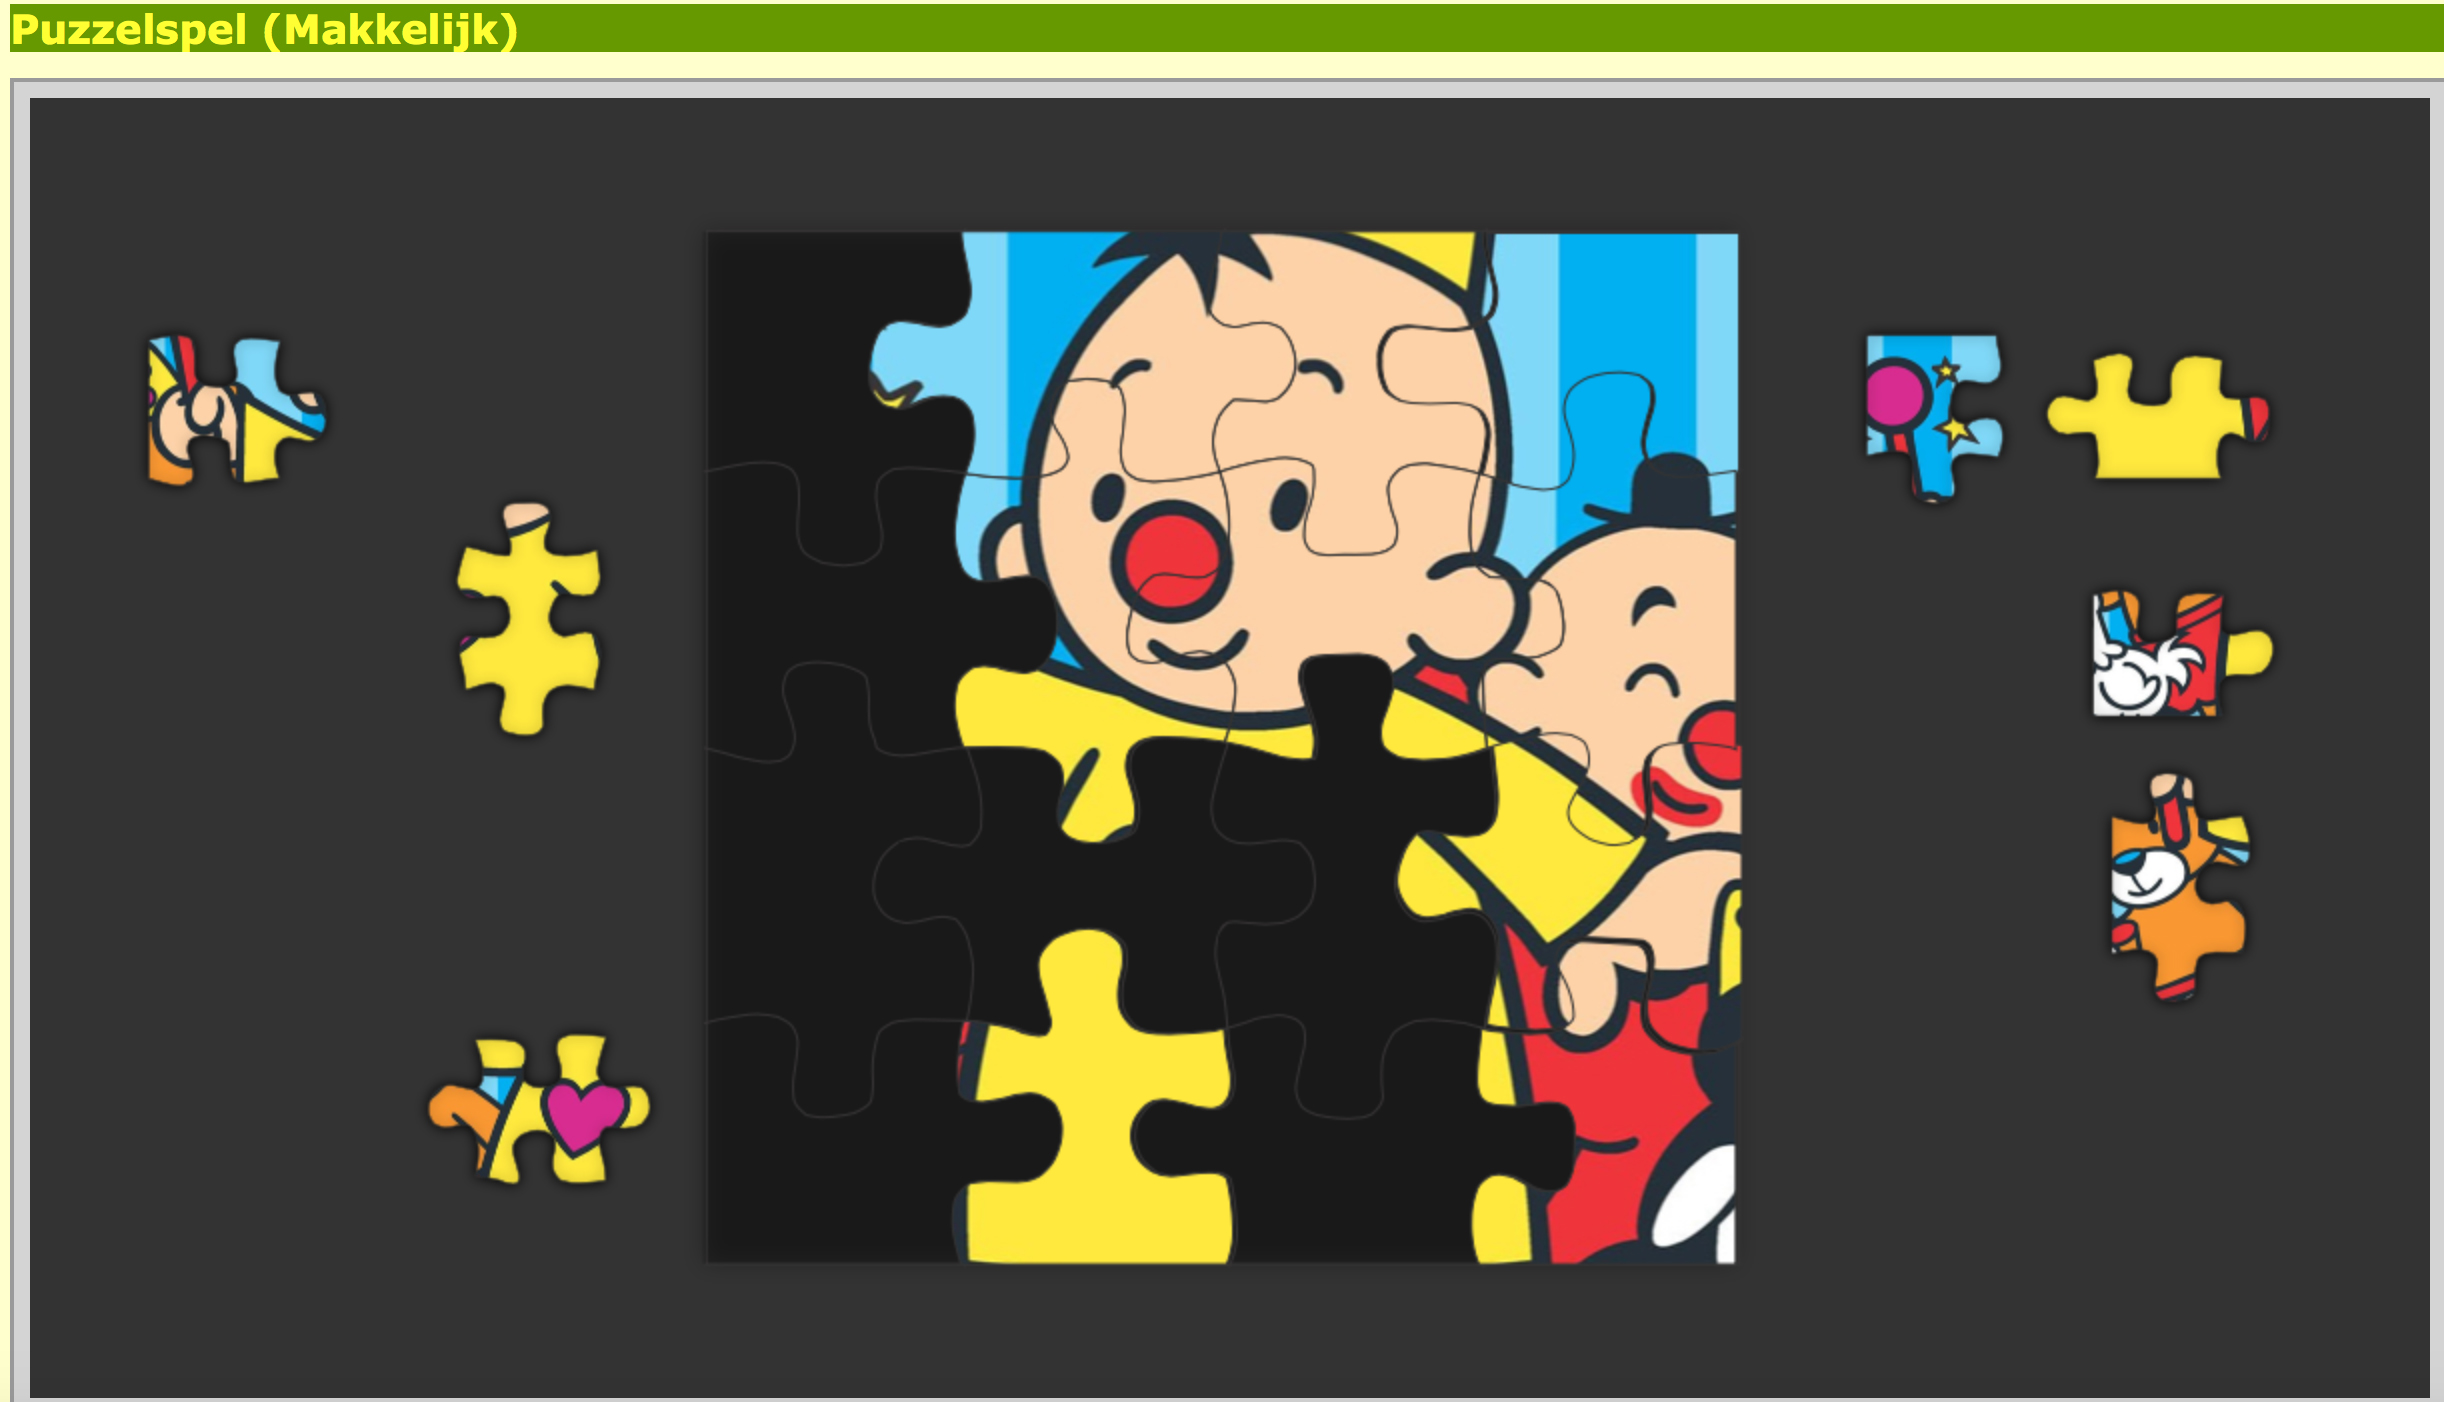
\includegraphics[scale=0.085]{bumba.jpg}
                \caption{Een makkelijke puzzel.}
                \label{bumba}
        \end{subfigure}%
        \begin{subfigure}{.5\textwidth}
           \centering
                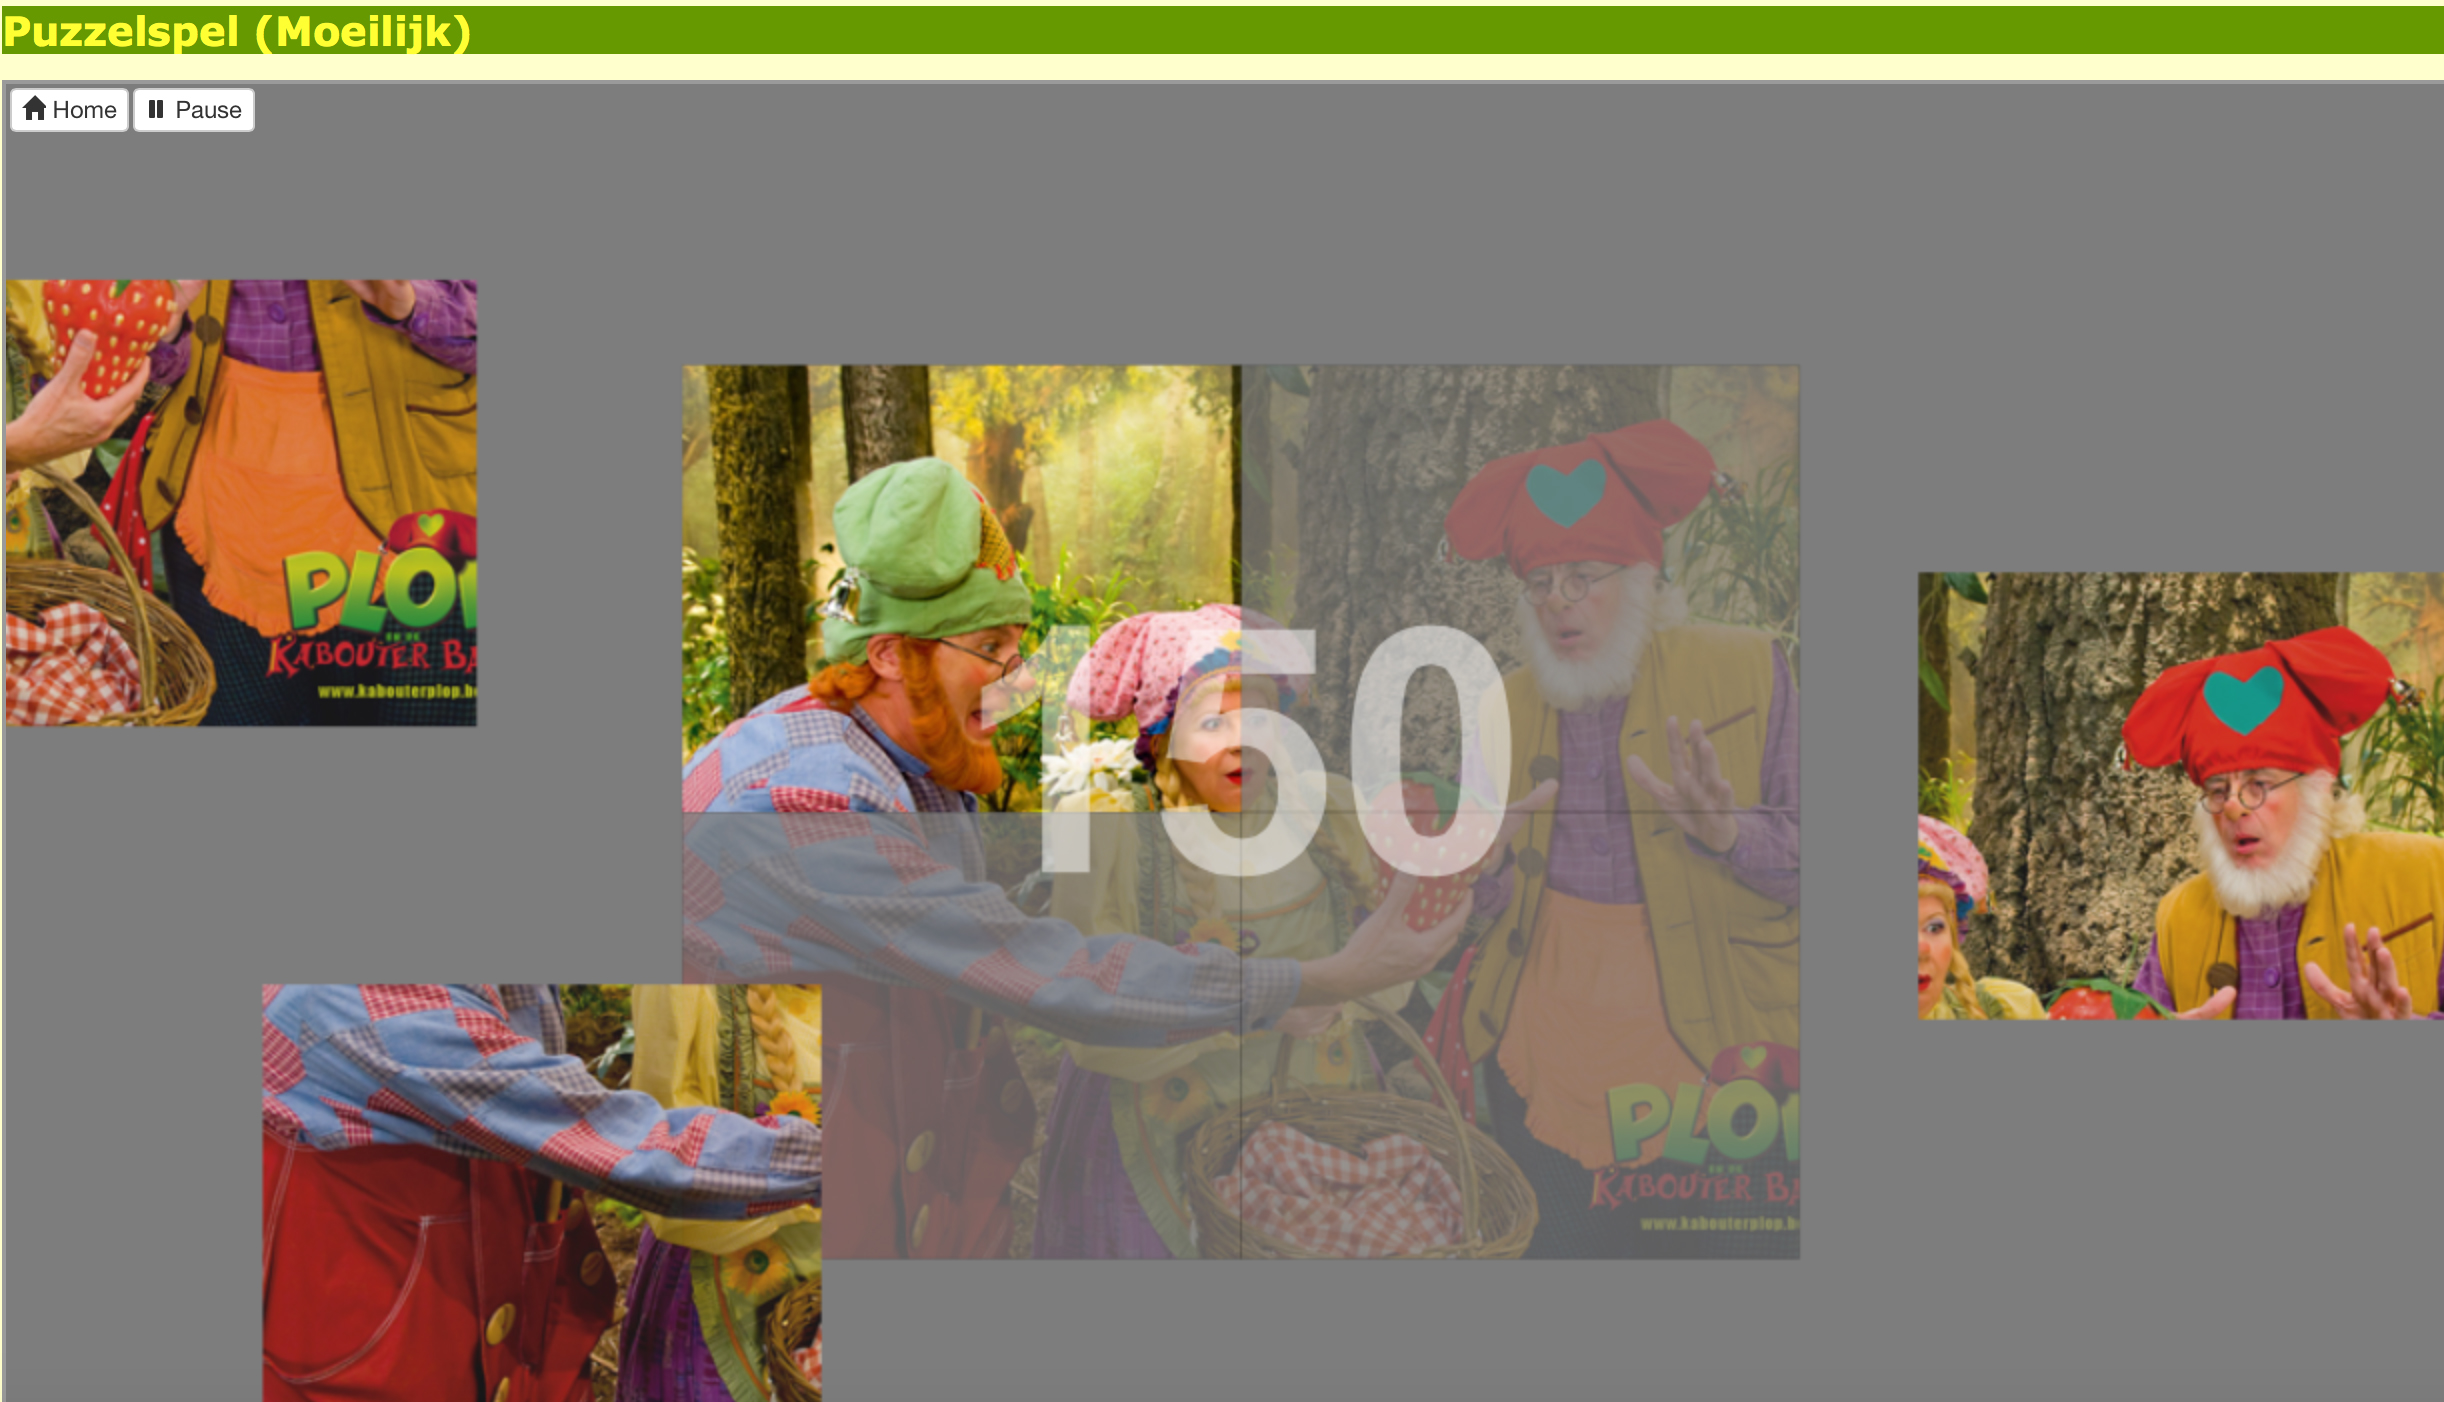
\includegraphics[scale=0.085]{mpuzzel.jpg}
                \caption{Een moeilijke puzzel met meerdere levels.}
                \label{mpuzzel}
        \end{subfigure}
        \begin{subfigure}{1\textwidth}
           \centering
                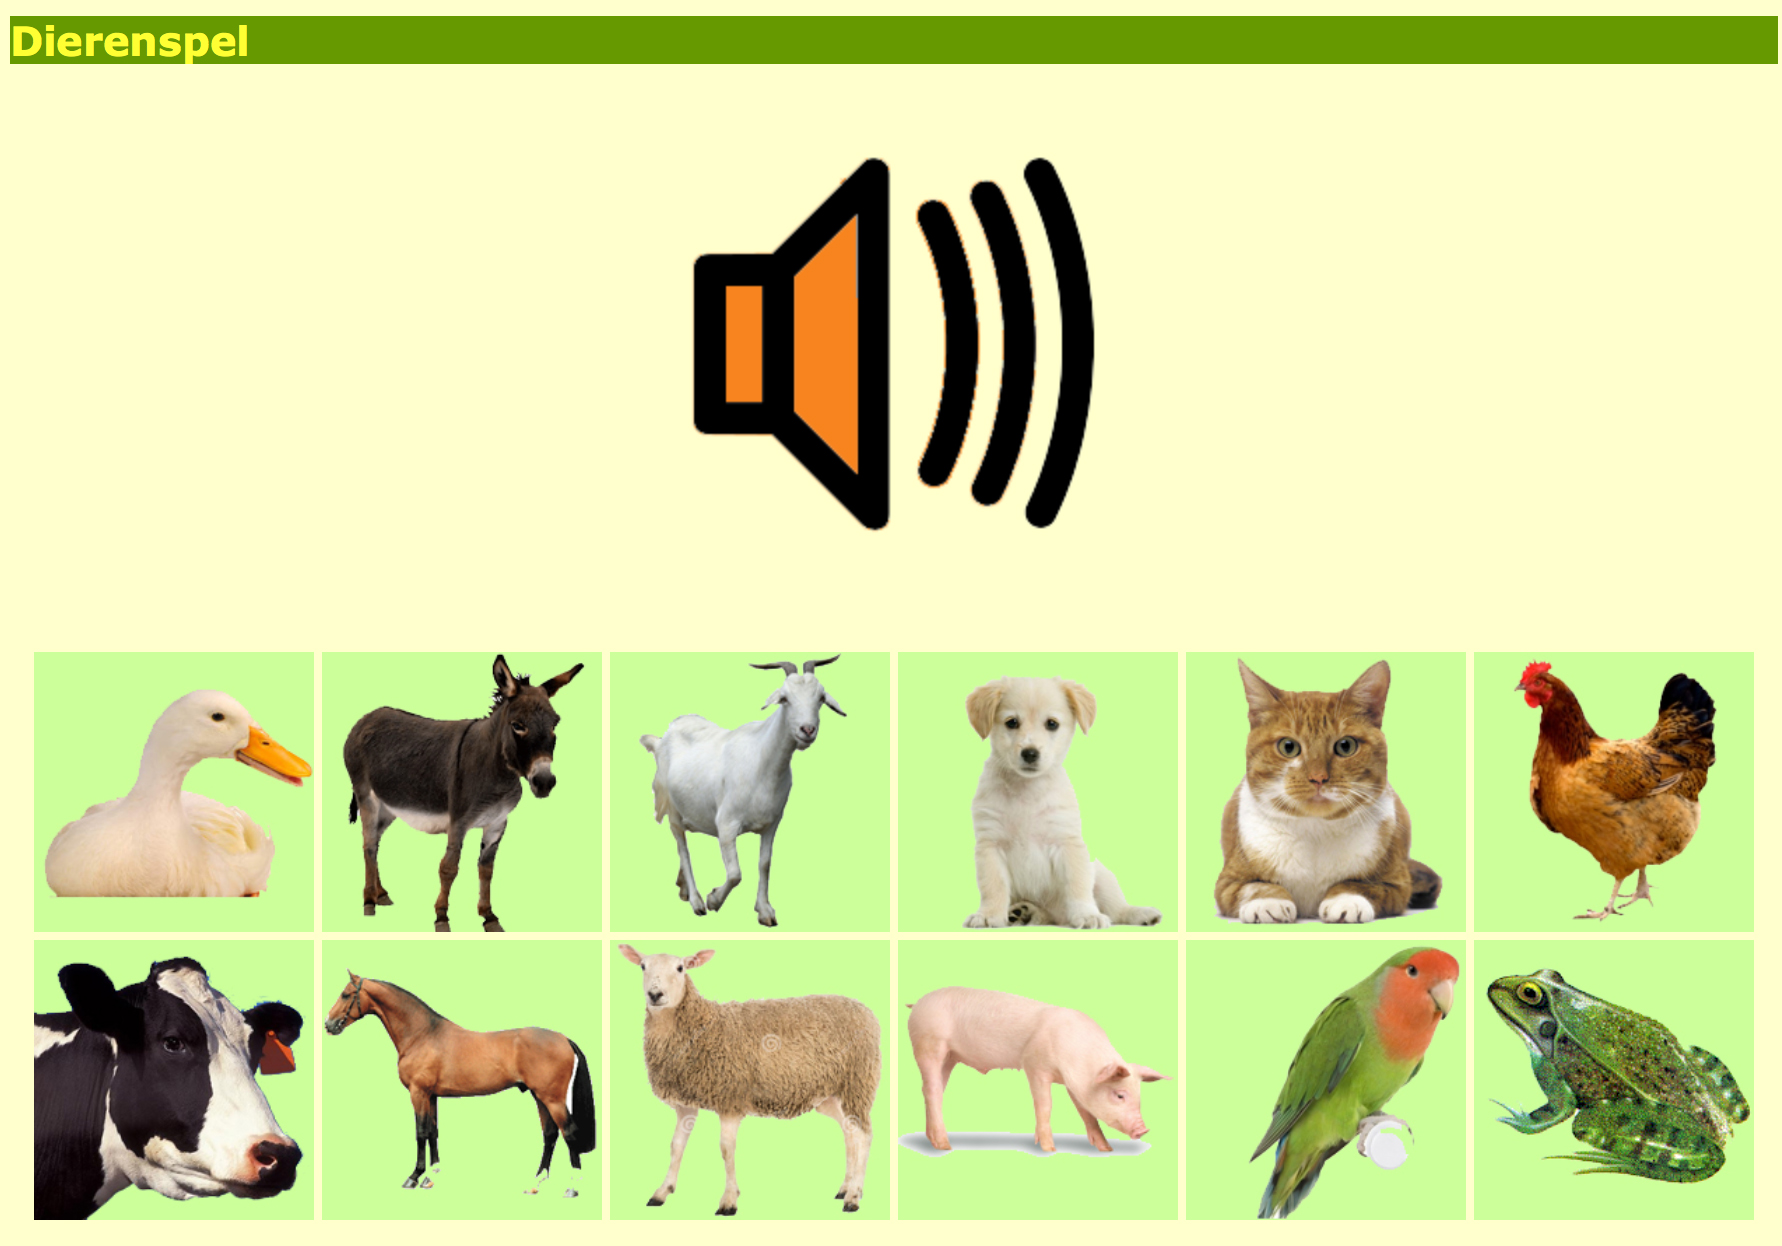
\includegraphics[scale=0.15]{dieren.jpg}
                \caption{Het dierenspel.}
                \label{dieren}
        \end{subfigure}
           \caption{Screenshots van de ICT-toepassingen ontwikkeld voor de oriëntatieklas van Elke Van Hout.}
\end{figure}
Wegens het erg grote niveauverschil, was het erg moeilijk om hier algemene 
richtlijnen te verkrijgen over wat leerlingen wel en niet kunnen. Vandaar ook de 
keuze om zowel een heel makkelijke als een veel moeilijkere puzzel te 
ontwikkelen. Sommige leerlingen in de klas kunnen immers maximaal een `echte' puzzel van 
20 stukken oplossen, anderen slagen erin om een puzzel van om en bij de 70 
stukken tot een goed einde te brengen. Ook voor het dierenspel waren er geen 
algemene richtlijnen beschikbaar.\\

\noindent Het testen vond plaats tijdens mijn laatste stagedag op de 
heemschool met enkele leerlingen apart. Al snel viel op dat de moeilijke puzzel 
met meerdere levels ook gewoon te moeilijk was. Na de tweede level kon geen 
enkele leerling nog binnen de tijdslimiet de puzzel oplossen. In de finale 
eindversie heb ik daarom de tijdslimiet enorm opgetrokken bij alle levels en ook 
gezorgd dat de eerste levels zeer, zeer eenvoudig beginnen zodat alle leerlingen 
toch een redelijke vooruitgang in het puzzelspel kunnen boeken. \\

\noindent In deze klas zat er ook een leerling met een motorische beperking 
waardoor de besturing van de muis via een soort joystickmuis verloopt (zie Figuur 
\ref{joy}). Deze joystickmuis gedraagt zich als een doodgewone muis op een 
computer, de bediening is alleen veel aangepaster aan de gebruiker met een 
motorische beperking (een joystick is veel makkelijker te hanteren dan een muis in gevallen van spierslapte en/of spastische neigingen). 
De 4 knoppen dienen ter vervanging van één keer klikken op de linkermuisknop, één 
keer klikken op de rechtermuisknop, dubbelklikken op de linkermuisknop en 
dubbelklikken op de rechtermuisknop.
Deze leerling maakt echter regelmatig onverwachte en ongecontroleerde 
bewegingen, waardoor de joystickmuis bewust is ingesteld om zeer traag over het 
scherm te rollen. Voor hem was dan ook de makkelijke puzzel en het dierenspel 
het enige haalbare om te doen. De moeilijke puzzel was met zijn meerdere levels 
en tijdslimieten onhaalbaar met de traag ingestelde joystickmuis.
 \begin{figure}[h!]
  \centering
  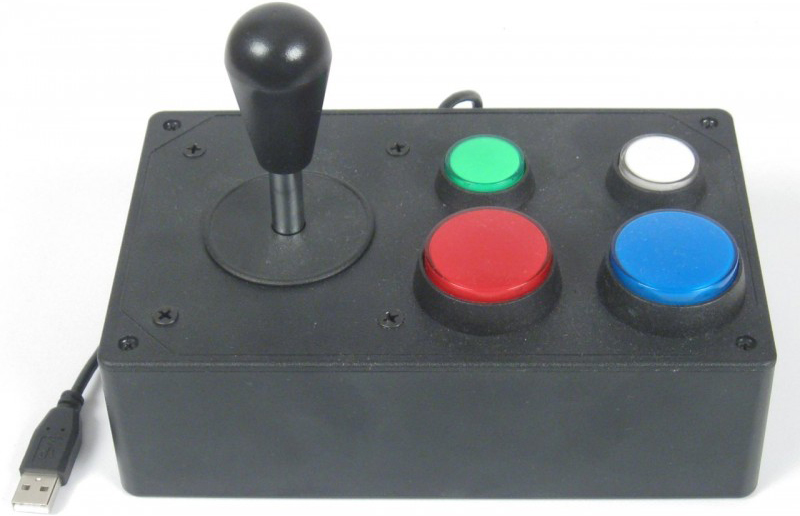
\includegraphics[scale=0.25]{joy.jpg}\caption{Een joystickmuis ter vervanging van een reguliere muis voor mensen met een motorische beperking. De rode knop komt overeen met één keer klikken op de linkermuisknop, de groene knop met dubbelklikken op de linkermuisknop. Analoog voor de blauwe en witte knop, zij vervangen de rechtermuisknop.}\label{joy}
\end{figure}


\subsection{Het eindresultaat}
Vermits de computerinfrastructuur op de stageschool erg beperkt was met veel oude computers, wou ik echt dat mijn materiaal 
zo gemaakt werd dat het ook op deze infrastructuur probleemloos kon draaien. Op 
het einde van de stage werd ook al het materiaal aan alle leerkrachten van de 
heemschool (ook diegenen die geen oproep hadden gedaan om ICT-materiaal te ontwikkelen) 
bezorgd via een afsluitend bericht op Smartschool (zie Figuur \ref{einde}).
\begin{figure}
  \centering
  
\includegraphics[scale=0.27]{eindoproep.jpg}\caption{Het slotbericht aan alle leerkrachten van de Heemschool werd op Smartschool gepubliceerd.}\label{einde}
\end{figure}

\subsubsection{Website}
In eerste instantie heb ik daarom alle oefeningen gemaakt als webpagina, zodat de leerkrachten 
gewoon naar een website moeten surfen om de oefeningen te kunnen starten. Dat 
vermijdt dat de leerkrachten software moeten installeren op de computer, naar 
een website surfen is voldoende. Een screenshot van de website kan je vinden op Figuur \ref{website}\\

\noindent\framebox(440, 30){ 
\parbox{430\unitlength}{\centering Op de website \textbf{www.filipmoons.com/heemschool} kan je alle oefeningen uittesten.}
}

 \begin{figure}[h!]
  \centering
  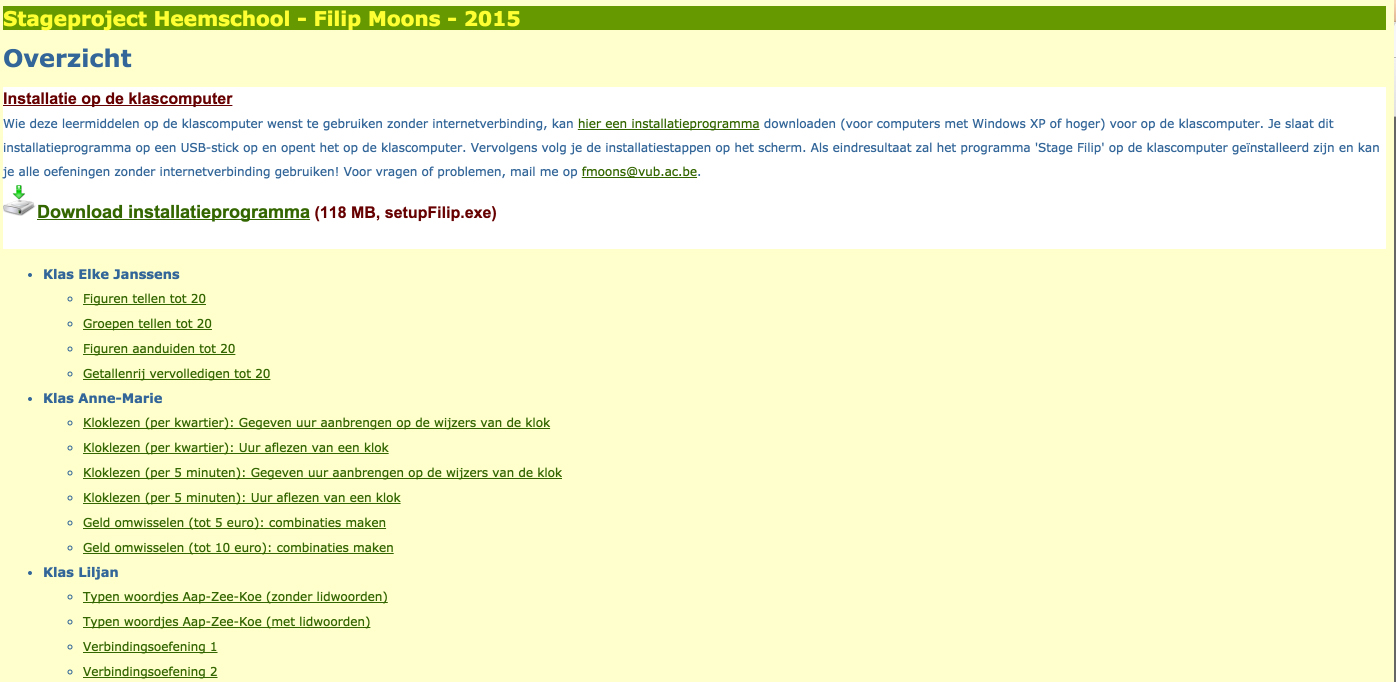
\includegraphics[scale=0.25]{website.jpg}\caption{De website www.filipmoons.com/heemschool bundelt alle oefeningen.}\label{website}
\end{figure}
\subsubsection{Installatieprogramma}
Hoewel initieel niet gepland, heb ik op vraag van de leerkrachten ook een installatieprogramma gemaakt 
zodanig dat leerkrachten de leermiddelen kunnen installeren op de klascomputer zonder daarbij een internetverbinding nodig te hebben. 
Het installatieprogramma installeert de oefeningen zoals een normaal programma op 
de computer.
De vraag is er gekomen omdat de meeste computers in de klassen geen of een erg onbetrouwbare 
internetverbinding hebben.  Het installatieprogramma werkt voor 
computers met Windows XP of hoger. Een screenshot vind 
je in Figuur \ref{installatie}. Ook het installatieprogramma kan je afhalen via 
de website \textbf{www.filipmoons.com/heemschool}. Een leerkracht die het 
programma dan op de internetloze klascomputer wil installeren, kan eenvoudigweg het 
installatieprogramma op een USB-stick zetten en het installatieprogramma openen op de klascomputer.

\begin{figure}[h!]
        \centering
        
        \begin{subfigure}{1\textwidth}
          \centering
                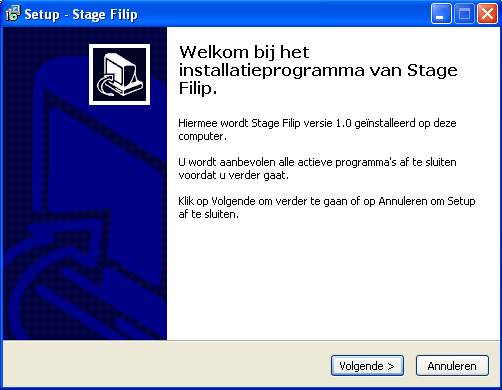
\includegraphics[scale=0.5]{installatie.png}
                \caption{De installatieprocedure installeert de oefeningen op een klascomputer op een alomgekende manier.}
        \end{subfigure}%
        \\
        \quad
        \\
        
        \begin{subfigure}{1\textwidth}
           \centering
                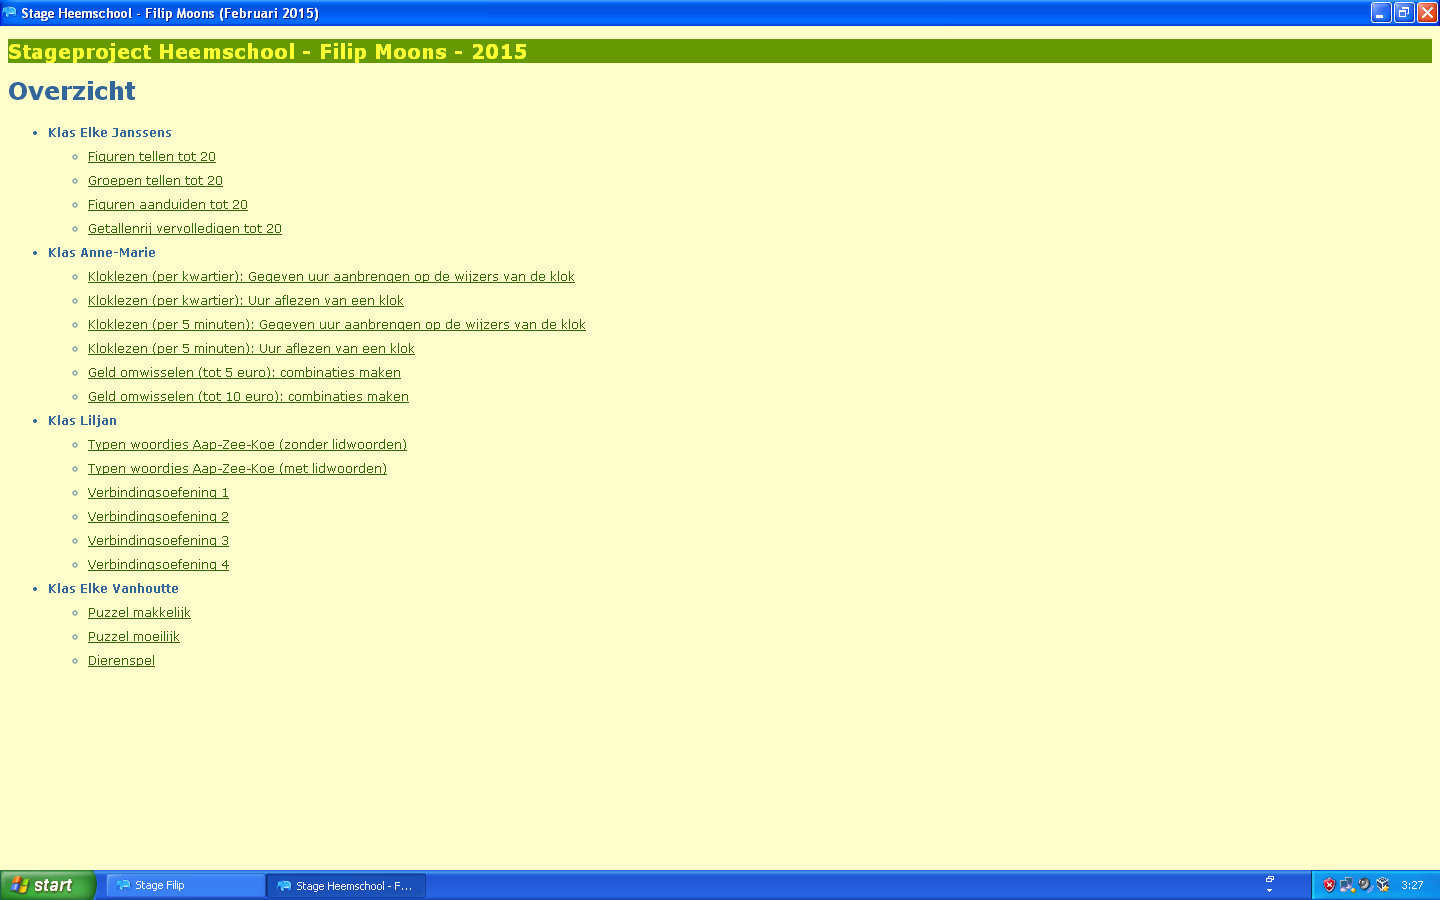
\includegraphics[scale=0.3]{normaalprogramma.png}
                \caption{De oefeningen draaien nu als een normaal programma op de klascomputer.}
        \end{subfigure}
        
           \caption{Via een installatieprocedure kan je de oefeningen ook als een gewoon programma installeren waarvoor je geen internetverbinding nodig hebt.}\label{installatie}
\end{figure}
\clearpage
\section{Logboek}\label{logboek}
De stage valt uiteen in twee delen: twee observatieweekjes en een testweek waarin ik het ontwikkeld ICT-materiaal samen
met de leerlingen getest heb. De twee delen werden bewust gescheiden door de krokusvakantie, zodanig dat ik voldoende tijd had 
om de digitale leermiddelen te maken. De observaties worden meer gedetailleerd besproken in sectie \ref{observaties} en de ontwikkeling
van het ICT-materiaal wordt besproken onder \ref{project}. De gepresteerde uren waarin ik 
individueel thuis de computertoepassingen ontwikkeld heb staan steeds schuin 
aangegeven.
\subsection{Observaties}
\begin{itemize}
  \item \textbf{Dinsdag 3 februari 2014}: Hele schooldag (09.00u-15.30u) 
  geobserveerd.
    \begin{itemize}
    \item \textbf{09.00-09.50}:   Observatie van een les rond boodschappen doen bij Heemklas 3 bij Anne-Marie,
    \item \textbf{09.50-10.40}:   Observatie van een verhaal bij de `zwakke' Eindklas 1 bij Wendy,
    \item \textbf{10.40-11.00}:   Speeltijd,
     \item \textbf{11.00-12.40}:  Observatie van een typles waarbij leerlingen hun naam moeten schrijven op de computer bij de `zwakke' Eindklas 1 bij Wendy,
    \item \textbf{12.40-13.50}:   Middagpauze,
    \item \textbf{13.50-14.40}:   Observatie van een geluidsles bij de autiklasjes bij An,
    \item \textbf{14.40-15.30}:   Observatie van een tekenles bij de `zwakke' Eindklas 1 bij Wendy. 
    \item \textbf{Avond}: Oproep gelanceerd op Smartschool voor alle 
    leerkrachten om ICT-materiaal dat ze graag ontwikkeld zouden zien naar mij 
    door te sturen.
  \end{itemize}
  \item \textbf{Vrijdag 6 februari 2014}: (Bijna) hele schooldag (09.00u-15.30u) 
  geobserveerd.
    \begin{itemize}
    \item \textbf{09.00-09.50}:   Observatie van een les rond het starten van de dag (welke dag is het vandaag, welke dag is het morgen, welke maand,...) bij Observatieklas 1 bij Elke Van Hout,
    \item \textbf{09.50-10.40}:   Observatie bij de logopediste Martine rond het verschil van smaken leren herkennen bij een Heemschool 1 klasje. Leerlingen herkenden het verschil tussen suiker en zout niet, 
    \item \textbf{10.40-11.00}:   Speeltijd,
    \item \textbf{11.00-12.40}:   Observatie van een les rond inlevingsvermogen bij de Heemklas 2 bij Elke Janssens. De les werd samen met de logopediste Martine gegeven,
    \item \textbf{12.40-13.50}:   Middagpauze,
    \item \textbf{13.50-14.40}:   Observatie van een les rond het aankleden bij de Observatieklas 1 bij Elke Van Hout.  \end{itemize}
 \end{itemize}
  \item \textbf{Woensdag 11 februari 2014} Halve schooldag geobserveerd (09.00u-12.40u)
   \begin{itemize}
    \item \textbf{09.00-09.50}:   Observatie van een les logopedie in de Heemklas 2 van Elke Janssens. Leerlingen moeten aan de hand 
    van afbeeldingen (bv. een afbeelding van twee kinderen die aan het vechten zijn) voorspellen wat er gaat gebeuren,
    \item \textbf{09.50-10.40}:   Observatie van een schrijfles bij de Heemklas 2 van Elke Janssens. Vervolgens gingen we ook naar de computerklas waar de leerlingen hun naam en adres moeten leren typen.  
    \item \textbf{10.40-11.00}:   Speeltijd,
    \item \textbf{11.00-12.40}:   Logopediste laat me alle computertoepassingen zien waar zij gebruik van 
    maken in de school en de specifieke software (zoals spraakcomputers) die sommige leerlingen gebruiken.
 \end{itemize}
   \item \textbf{Donderdag 12 februari 2014} Hele schooldag (09.00u-15.30u) 
  geobserveerd.
    \begin{itemize}
    \item \textbf{09.00-10.40}:   Observatie van een les rond het starten van de dag (alle klassen starten hiermee) in de  
    `sterke' Eindklas 2 van Kathleen. Daarna ging de les over technisch reken: 
    splitsen van tientallen en eenheden. Dit zijn echt lessen op het hoogste 
    niveau in de heemschool. 
    \item \textbf{10.40-11.00}:   Speeltijd,
    \item \textbf{11.00-12.40}:   Observatie in het autiklasje waarbij ook afspraken gemaakt werden voor het ontwikkelen van ICT-materiaal voor de autileesmethode`Aap-Zee-Koe'. 
    Na de afspraken heb ik nog een muzieklesje gevolgd waarbij de leerlingen 
    allerlei aangeleerde danslesjes deden.
   \item \textbf{12.40-13.50}:   Middagpauze,
    \item \textbf{13.50-15.30}:   Individuele afspraken gemaakt met Anne-Marie (Heemklas 3), Elke Janssens (Heemklas 2) en Elke Van Hout (Observatieklas 1) rond de ontwikkeling
    van mijn ICT-materiaal.
     \end{itemize}

\end{itemize}
\subsection{Testweek}
\begin{itemize}
  \item \textbf{Zaterdag 21 februari 2015}:
  \begin{itemize}
    \item \textbf{Hele dag}: \emph{ Ontwikkeling ICT-materiaal (voor tellen tot 20, kloklezen en geld wisselen)
  voor Elke Janssens (Heemklas 2) en Anne-Marie (Heemklas 3).}
  \end{itemize}

  

   \item \textbf{Zondag 22 februari 2015}:  \begin{itemize}
    \item \textbf{Hele dag}: \emph{ Ontwikkeling ICT-materiaal (voor tellen tot 20, kloklezen en geld wisselen)
  voor Elke Janssens (Heemklas 2) en Anne-Marie (Heemklas 3).}
  \end{itemize}

  \item  \textbf{Dinsdag 24 februari 2014}:     
  \begin{itemize}
    \item \textbf{12.40-13.30}:   Afspraak met Anne-Marie (Heemklas 3) en Elke Janssens (Heemklas 2) om de ontwikkelde ICT-oefeningen voor te leggen
    en eventuele opmerkingen tot bijsturing te bekomen. Nadien getest in het computerlokaaltje of de oefeningen op de computers werken.
    \item \textbf{Avond}: \emph{ICT-oefeningen voor Heemklas 2 \& 3 (voor tellen tot 20, kloklezen en geld wisselen) bijgestuurd a.d.h.v. gegeven opmerkingen.}
  \end{itemize}
  
  \item  \textbf{Woensdag 25 februari 2014}:     
  \begin{itemize}
    \item \textbf{09.00-09.50}:   ICT-oefeningen getest met de Heemklas 3 van Anne-Marie in het computerlokaaltje in aanwezigheid van stagebegeleider Evelyne De Smet.
     \item \textbf{09.50-10.20}:   ICT-oefeningen getest met de Heemklas 2 van Elke Janssens in het computerlokaaltje in aanwezigheid van stagebegeleider Evelyne De Smet.
     \item \textbf{Namiddag}: \emph{ICT-oefeningen ontwikkeld voor de autileesmethode `Aap-Zee-Koe'.}
  \end{itemize}
   \item  \textbf{Donderdag 26 februari 2014}:     
  \begin{itemize}
    \item \textbf{09.00-10.40}:   ICT-oefeningen rond de autileesmethode `Aap-Zee-Koe' getest met 2 leerlingen 
    van de autiklasjes    en nadien nog wat met hen gespeeld met foto-effecten op foto's van hen.
        \item \textbf{10.40-11.30}:  ICT-oefeningen ook lokaal op de 
        klascomputer geïnstalleerd en wat gebabbeld met de klasleerkracht 
        Liljan.
     \item \textbf{Namiddag:}: \emph{ICT-oefeningen (puzzels en dierenspel) ontwikkeld voor het observatieklasje van Elke Van Hout.}
     \end{itemize}
     \item  \textbf{Vrijdag 27 februari 2014}:     
  \begin{itemize}
    \item \textbf{09.00-10.40}:   ICT-oefeningen (puzzels en dierenspel) getest 
    met 2 leerlingen van het observatieklasje van Elke Van Hout.
   \item \textbf{10.40-13.30}:  Nog enkele uitbreidingen besproken die Anne-Marie gevraagd had. 
   Vervolgens afscheid genomen van alle leerkrachten en leerlingen.
   \end{itemize}
   
 \item \textbf{Zondag 29 februari 2015}:  
 \begin{itemize}
    \item \textbf{Voormiddag}: \emph{Uitbreidingen afgewerkt en alle foutjes die opdoken tijdens het testen met de leerlingen hersteld in de ICT-oefeningen. Vervolgens
    naar alle leerkrachten het eindresultaat gemaild.}
    
  \end{itemize}
  \end{itemize}
  
  
\end{itemize}

\newpage
\section{Slotconclusie en reflectieve beshouwing}
De stage op de Heemschool was écht een verbredende stage zoals beoogd door het 
vak: ik ben met een onderwijscontext in contact gekomen die ik voorheen niet 
kende en die ik waarschijnlijk zonder deze stage ook nooit zou leren kennen. 
Zeker 

\newpage
\section{Bibliografie}
\begin{itemize}
  \item V. Soetewey (2009). \emph{Cursus: Bijzondere Doelgroepen}. Crefi. 
  \item S. Mignon (2011). \emph{Het syndroom van Pradar-Willi}. Masterthesis tot behalen van de graad `Dokter in de Geneeskunde', Vrije Universiteit Brussel. 

    \item J. De Witte (2013). \emph{Met een handicap naar de school van je keuze. Redelijke 
    aanpassingen in het onderwijs}. Brussel: Centrum voor gelijkheid van kansen en voor 
    racismebestrijding.
   \item L. Phipps, A. Sutherland, J Seale (eds.) (2002).  \emph{Access all areas: disability, technology and learning}. York, UK: TechDis with the Association for Learning 
   Technology.
   

\end{itemize}
\newpage
\section{Bijlagen}
Een kopie van de stageovereenkomst zal in de afgedrukte versie van dit 
stagerapport toegevoegd worden. De afgedrukte versie wordt overhandigd tijdens 
de mondelinge presentatie.
\cftaddtitleline{toc}{subsection}{1.\;\;\;\; Kopie van de stageovereenkomst}{A}


 \end{document}

